\documentclass[a4paper,12pt]{article}
\usepackage[utf8]{inputenc}

\usepackage{amsmath}

\usepackage[T1]{fontenc}
\usepackage[english, polish]{babel}
\usepackage[utf8]{inputenc}
\usepackage{tikz}
\usetikzlibrary{conceptgraph}

\newcommand{\sg}{{\it sg} }
\newcommand{\pl}{{\it pl} }
\newcommand{\mass}{{\it mass} }
\newcommand{\ind}{{\it indexical} }
\newcommand{\corf}{{\it coreferential} }
\newcommand{\deict}{{\it deictic} }
\newcommand{\interr}{{\it interrogative} }

\title{Koncepcja metaopisu semantycznego}
\author{Wojciech Jaworski}
\date{}

\begin{document}

\maketitle

\section{Wprowadzenie}

Znaczenie wypowiedzeń reprezentowane jest w systemie dwupoziomowo.
Najpierw za pomocą grafu semantycznego opisującego występujące w tekście pojęcia
oraz relacje pomiędzy nimi a następnie w postaci formuły logiki pierwszego rzędu
rozszerzonej o predykat metajęzykowy i dodatkowe kwantyfikatory.

Różnica pomiędzy reprezentacjami polega na tym, że
graf semantyczny jest bliższy składni, natomiast formuła logiczna posiada formalnie zdefiniowaną semantykę.
Formuła logiczna jest generowana z grafu semantycznego za pomocą algorytmu, co pozwala przenieść
formalną semantykę na graf. Niniejszy dokument skupia się na opisie poszczególnych zjawisk językowych za pomocą grafów semantycznych.

Grafy semantyczne inspirowane są pracami Johna Sowy (`` Knowledge Representation:
Logical, Philosophical, and Computational Foundations'')

Podstawy reprezentacji zostały opracowane w ramach projektu Clarin i
są opisane w dokumencie: ``Język reprezentacji znaczenia dla języka
polskiego'' oraz szkicowo opublikowane na konferencji COLING 2016 w 
pracy ``ENIAM: Categorial Syntactic-Semantic Parser for Polish''.
Poniżej zostanie opisane sposób w jaki poszczególne zjawiska składniowe 
są reprezentowane za pomocą grafów pojęć. Opis ma charakter techniczny 
i nie obejmuje rozważań dotyczących teoriomodelowej semantyki poszczególnych konstrukcji, 
analizy możliwych reprezentacji ani kontekstów literaturowych. 
Celem, oprócz opisania zasad tworzenia form logicznych przez parser ENIAM
jest określenie formatu zasobów leksykalnych potrzebnych do ich wygenerowania.

\section{Pojęcia i relacje między pojęciami}
Formuły naszego języka reprezentacji znaczenia wyrażamy graficznie
w formie grafów semantycznych. % równoważnych tradycyjnie rozumianym formułom logicznym.
Przykładowo dla zdania {\it Słoń trąbi} uzyskamy graf 

\[\begin{tikzpicture}
\node[concept] (t) {trąbić};
\node[relation, right=1cm of t] (ts) {Init};
\node[concept, right=1cm of ts] (s) {\sg słoń};
\node[relation, left=1cm of t] (pr) {Pres};
\context{cx}{(t)(ts)(s)}{};
\edge {t} {ts};
\edge {cx} {pr};
\edge {ts} {s};
\end{tikzpicture}\]

W powyższym grafie pudełka reprezentują obiekty, o których jest mowa.
Występuje zatem obiekt {\it słoń} i zdarzenie {\it trąbić}.
Symbol $\sg$ określa liczność obiektów jako dokładnie 1.

Kółeczka reprezentują relacje między obiektami.
Init wskazuje na to, że {\it słoń} jest inicjatorem {\it trąbienia},
a Pres na to, że zdarzenie jest równoczesne z czasem jego wypowiedzenia.
%TODO unaukowić i zrobić opis semantyczny czasu 
Strzałka wchodząca to pierwszy argument, wychodząca drugi.
Źródłem informacji o relacjach łączących czasowniki 
(a w przyszłości również rzeczowniki, przymiotniki i przysłówki) z ich argumentami jest słownik walencyjny Walenty.

Zewnętrzna ramka to kontekst. Reprezentuje on sytuację, czyli 
podzbiór czasoprzestrzeni, w którym istnieją byty wskazane przez pojęcia w pudełkach
i zachodzą wymienione w kółeczkach relacje pomiędzy nimi.

Standardowo każdej jednostce leksykalnej (leksemowi lub wyrażeniu wielosłownemu) 
zawartej w zdaniu odpowiada pudełko, a relacji składniowej kółeczko.
Pudełka zawierają sensy jednostek leksykalnych oraz ich liczbę, a w przypadku 
nazw własnych nazwę i typ nazwy własnej np {\it Franciszek trąbi}:
\[\begin{tikzpicture}
\node[concept] (t) {trąbić};
\node[relation, right=1cm of t] (ts) {Init};
\node[concept, right=1cm of ts] (s) {\sg osoba ``Franciszek''};
\node[relation, left=1cm of t] (pr) {Pres};
\context{cx}{(t)(ts)(s)}{};
\edge {t} {ts};
\edge {cx} {pr};
\edge {ts} {s};
\end{tikzpicture}\]

\section{Wprowadzanie bytów do dyskursu}
W języku logiki pierwszego rzędu wzmiankowane byty stanowią odniesienia zmiennych, a
same zmienne wprowadzane są przez kwantyfikatory. Przy czym dostępne są dwa rodzaje kwantyfikacji:
uniwersalna w której wartościowanie wprowadzanej zmiennej przebiega po wszystkich elementach uniwersum
spełniających restrykcję oraz egzystencjalna, przy której zmienna wartościowana jest jednym 
z bytów spełniających restrykcję.

W przypadku grafów semantycznych zmienne nie są jawnie wskazane, tym niemniej 
zachodzi konieczność określenia w jaki sposób obiekty wskazywane przez pudełka 
są wiązane z uniwersum.

Domyślnie przyjmujemy kwantyfikację egzystencjalną, czyli np. zdanie {\it Słoń trąbi}
stwierdza o istnieniu {\it słonia} i istnieniu zdarzenia {\it trąbienia}.

Z kolei dla zdania {\it Ty biegniesz} otrzymamy reprezentację z pojęciem okazjonalnym (indexical),
który wiąże słowo {\it ty} z uczestnikami komunikacji, czyli odwołuje się do uniwersum na metapoziomie.
\[\begin{tikzpicture}
\node[concept] (t) {biec};
\node[relation, right=1cm of t] (ts) {Init};
\node[concept, right=1cm of ts] (s) {\ind ty};
\node[relation, left=1cm of t] (pr) {Pres};
\context{cx}{(t)(ts)(s)}{};
\edge {t} {ts};
\edge {cx} {pr};
\edge {ts} {s};
\end{tikzpicture}\]
a dla zdania {\it Ona biegnie} otrzymamy reprezentację z pojęciem deiktycznym 
\[\begin{tikzpicture}
\node[concept] (t) {biec};
\node[relation, right=1cm of t] (ts) {Init};
\node[concept, right=1cm of ts] (s) {\deict ona};
\node[relation, left=1cm of t] (pr) {Pres};
\context{cx}{(t)(ts)(s)}{};
\edge {t} {ts};
\edge {cx} {pr};
\edge {ts} {s};
\end{tikzpicture}\]
lub koreferencyjnym
\[\begin{tikzpicture}
\node[concept] (t) {biec};
\node[relation, right=1cm of t] (ts) {Init};
\node[concept, right=1cm of ts] (s) {\corf ona};
\node[relation, left=1cm of t] (pr) {Pres};
\context{cx}{(t)(ts)(s)}{};
\edge {t} {ts};
\edge {cx} {pr};
\edge {ts} {s};
\end{tikzpicture}\]
W powyższych trzech przypadkach nie następuje wprowadzenie nowego bytu do dyskursu.

Zaimki wnoszą informację o osobie, liczbie i rodzaju, która jest istotna przy ustalaniu ich referenta.
Z tego tego względu lematyzujemy je do form uwzględniających te informacje ({\it ja}, {\it wy}, {\it one}, {\it która}), ewentualnie uzupełniając 
np. {\it ja-m}.

Kiedy podmiot nie jest dany w sposób jawny, jest reprezentowany za pomocą wariantu niemego zaimka {\it pro}
np. {\it Biegnę}.:
\[\begin{tikzpicture}
\node[concept] (t) {biec};
\node[relation, right=1cm of t] (ts) {Init};
\node[concept, right=1cm of ts] (s) {\ind pro-ja};
\node[relation, left=1cm of t] (pr) {Pres};
\context{cx}{(t)(ts)(s)}{};
\edge {t} {ts};
\edge {cx} {pr};
\edge {ts} {s};
\end{tikzpicture}\]
Zaimek {\it pro} używany jest również, kiedy przedmiot jest wprowadzany poprzez podanie swojej cechy, 
co ma miejsce we frazach rzeczownikowych, których głową jest przymiotnik np. {\it Gruby trąbi.}
\[\begin{tikzpicture}
\node[concept] (t) {trąbić};
\node[relation, right=1cm of t] (ts) {Init};
\node[concept, right=1cm of ts] (s) {\ind pro-on};
\node[relation, left=1cm of t] (pr) {Pres};
\node[relation, right=10mm of s] (a) {Attr};
\node[concept, right=1cm of a] (b) {gruby};
\context{cx}{(t)(ts)(s)(a)(b)}{};
\edge {t} {ts};
\edge {cx} {pr};
\edge {ts} {s};
\edge {s} {a};
\edge {a} {b};
\end{tikzpicture}\]
Kolejnym zastosowaniem niemego zaimka są równoważniki zdań.
Dodajemy do nich {\it pro-zdarzenie}, które wiąże poszczególne elementy zdania,
np. {\it Kot pod stołem}
\[\begin{tikzpicture}
\node[concept] (a) {pro-zdarzenie};
\node[relation, left=1cm of a] (b) {Thme};
\node[concept, left=1cm of b] (c) {\sg kot};
\node[relation, above=0.8cm of a] (d) {Pres};
\node[relation, right=1cm of a] (e) {Loc};
\node[concept, right=1cm of e] (f) {pod};
\node[concept, below=0.5cm of e] (h) {\sg stół};
\context{cx}{(a)(b)(c)(e)(f)(h)}{};
\edge {a} {b};
\edge {b} {c};
\edge {cx} {d};
\edge {a} {e};
\edge [dashed]{e} {f};
\edge {e} {h};
\end{tikzpicture}\]
%TODO pro-zdarzenie to może też być stan, przydałaby się ogólniejsza nazwa



Leksemy {\it siebie} i {\it się} są koreferencyjne:
{\it Jan kupił sobie samochód}, {\it Jan myje się}
\[\begin{tikzpicture}
\node[concept] (t) {\sg osoba ``Jan''};
\node[relation, right=1cm of t] (ts) {Init};
\node[concept, right=1cm of ts] (s) {kupić};
\node[relation, left=1cm of t] (pr) {Pres};
\node[relation, right=1cm of s] (sk) {Rcpt};
\node[concept, right=1cm of sk] (k) {\corf siebie};
\node[relation, below=5mm of s] (a) {Thme};
\node[concept, right=1cm of a] (b) {\sg samochód};
\context{cx}{(t)(ts)(s)(sk)(k)(a)(b)}{};
\edge {ts} {t};
\edge {cx} {pr};
\edge {s} {ts};
\edge {s} {sk};
\edge {sk} {k};
\edge {s} {a};
\edge {a} {b};
\end{tikzpicture}\]
\[\begin{tikzpicture}
\node[concept] (t) {\sg osoba ``Jan''};
\node[relation, right=1cm of t] (ts) {Init};
\node[concept, right=1cm of ts] (s) {myć};
\node[relation, left=1cm of t] (pr) {Pres};
\node[relation, right=1cm of s] (sk) {Thme};
\node[concept, right=1cm of sk] (k) {\corf się};
\context{cx}{(t)(ts)(s)(sk)(k)}{};
\edge {ts} {t};
\edge {cx} {pr};
\edge {s} {ts};
\edge {s} {sk};
\edge {sk} {k};
\end{tikzpicture}\]

W dalszym toku tekstu wprowadzimy jeszcze pojęcia interrogatywne (interrogative),
występujące przy zadawaniu pytań, jak również kwantyfikację uniwersalną 
(przebiegającą po wielu bytach).
%kwantyfikacja uniwesalna może być wprowadzona niejawnie np: Słoń jest ssakiem, 

\section{Modyfikatory nieintersektywne}
Funkcja modyfikacji nieintersektywnej zachodzi między wyrażeniem określanym
a jego nieintersektywnym określnikiem, który może być przymiotnikiem 
({\it były prezydent}, {\it fałszywy brylant}, {\it sztuczny miód}), 
przysłówkiem ({\it pozornie zachodzi}) lub wyrażeniem przyimkowym ({\it je na niby}).
\[\begin{tikzpicture}
\node[concept] (a) {były(prezydent)};
\node[concept, right=1cm of a] (b) {fałszywy(brylant)};
\node[concept, right=1cm of b] (c) {sztuczny(miód)};
\end{tikzpicture}\]
\[\begin{tikzpicture}
\node[concept] (t) {pozornie(zachodzić)};
\node[relation, right=1cm of t] (ts) {Thme};
\node[concept, right=1cm of ts] (s) {\deict pro-3sg};
\node[relation, left=1cm of t] (pr) {Pres};
\context{cx}{(t)(ts)(s)}{};
\edge {t} {ts};
\edge {cx} {pr};
\edge {ts} {s};
\end{tikzpicture}\]
\[\begin{tikzpicture}
\node[concept] (t) {na niby(jeść)};
\node[relation, right=1cm of t] (ts) {Init};
\node[concept, right=1cm of ts] (s) {\deict pro-3sg};
\node[relation, left=1cm of t] (pr) {Pres};
\context{cx}{(t)(ts)(s)}{};
\edge {t} {ts};
\edge {cx} {pr};
\edge {ts} {s};
\end{tikzpicture}\]
% prawie [prawie:qub] 	dobiegłem do mety\\
% broda pokrywała 	prawie [prawie:qub] 	całą jego twarz\\

%TODO: Kryteria określające, kiedy przymiotnik stanowi fragment jednostki wielosłownej, kiedy zmienia znaczenie rzeczownika, a kiedy wyznacza jego cechy.

\section{Liczebność i miara}

Liczebność odniesienia rzeczowników policzalnych wskazuje relacja Count,
np: {\it Dwa słonie trąbią}, {\it trzy i pół jabłka}, {\it kilka słoni}
\[\begin{tikzpicture}
\node[concept] (t) {trąbić};
\node[relation, right=1cm of t] (ts) {Init};
\node[concept, right=1cm of ts] (s) {słoń};
\node[relation, left=1cm of t] (pr) {Pres};
\node[relation, right=1cm of s] (sk) {Count};
\node[concept, right=1cm of sk] (k) {2};
\context{cx}{(t)(ts)(s)(sk)(k)}{};
\edge {t} {ts};
\edge {cx} {pr};
\edge {ts} {s};
\edge {s} {sk};
\edge {sk} {k};
\end{tikzpicture}\]
\[\begin{tikzpicture}
\node[concept] (t) {jabłko};
\node[relation, right=1cm of t] (ts) {Count};
\node[concept, right=1cm of ts] (s) {3.5};
\edge {t} {ts};
\edge {ts} {s};
\end{tikzpicture}\]
\[\begin{tikzpicture}
\node[concept] (t) {słoń};
\node[relation, right=1cm of t] (ts) {Count};
\node[concept, right=1cm of ts] (s) {kilka};
\edge {t} {ts};
\edge {ts} {s};
\end{tikzpicture}\]
{\it między 2 a 5 jabłek}
\[\begin{tikzpicture}
\node[concept] (a) {2};
\node[concept, right=5mm of a] (b) {5};
\context{v}{(a)(b)}{a};
\node[relation, right=10mm of b] (f) {Count};
\node[concept, below=5mm of f] (e) {między};
\node[concept, right=10mm of f] (g) {jabłko};
\edge{f}{v};
\edge[dashed]{f}{e};
\edge{g}{f};
\end{tikzpicture}\]
{\it 3 lub 4 jabłka}
\[\begin{tikzpicture}
\node[concept] (a) {3};
\node[concept, right=5mm of a] (b) {4};
\context{v}{(a)(b)}{lub};
\node[relation, right=10mm of b] (f) {Count};
\node[concept, right=10mm of f] (g) {jabłko};
\edge{f}{v};
\edge{g}{f};
\end{tikzpicture}\]
Liczebniki określone reprezentujemy za pomocą liczb, a nieokreślone (np {\it kilka, trochę}) za pomocą leksemów.
Dwa ostatnie z powyższych przykładów wykorzystuj notację dla koordynacji opisaną szczegółowo w rozdziale \ref{coordination}.

Liczebniki mogą być modyfikowane przez operatory adnumeratywne np. {\it prawie 30 słoni}.
\[\begin{tikzpicture}
\node[concept] (t) {jabłko};
\node[relation, right=1cm of t] (ts) {Count};
\node[concept, right=1cm of ts] (s) {30};
\node[concept, below=0.5cm of ts] (a) {prawie};
\edge {t} {ts};
\edge {ts} {s};
\edge [dashed]{ts} {a};
\end{tikzpicture}\]
Podobnie zachowują się {\it około}, {\it koło}, {\it co najmniej}, {\it niemal}, {\it niespełna}, {\it co najwyżej}, {\it ponad}, {\it prawie}, {\it przeszło}, {\it przynajmniej}.

Liczność rzeczowników, które nie mają jej jawnie zadanej przez liczebnik
wnioskujemy na podstawie liczby gramatycznej i zapisujemy za pomocą uproszczonej notacji.
Symbol $\sg$ określa liczność obiektów jako dokładnie 1.
\[\text{Graf }\begin{tikzpicture}
\node[concept] (t) {\sg słoń};
\end{tikzpicture}
\text{ jest równoważny }
\begin{tikzpicture}
\node[concept] (t) {słoń};
\node[relation, right=1cm of t] (ts) {Count};
\node[concept, right=1cm of ts] (s) {1};
\edge {t} {ts};
\edge {ts} {s};
\end{tikzpicture}\]

Oprócz niego stosujemy symbol $\pl$ na określenie liczności większej niż 1.
\[\text{Graf }\begin{tikzpicture}
\node[concept] (t) {\pl słoń};
\end{tikzpicture}
\text{ jest równoważny }
\begin{tikzpicture}
\node[concept] (t) {słoń};
\node[relation, right=1cm of t] (ts) {Count};
% \node[concept, right=1cm of ts] (s) {co najmniej(2)};
\node[concept, right=1cm of ts] (s) {1};
\node[concept, below=0.5cm of ts] (a) {ponad};
\edge {t} {ts};
\edge {ts} {s};
\edge [dashed]{ts} {a};
\end{tikzpicture}\]
Rzeczowniki plurale tantum nie wnoszą informacji o liczności.

Dla innych części mowy liczność uznajemy za nieokreśloną, gdy nie jest jawnie wskazana.
Liczebność czasowników wskazuje zazwyczaj leksem {\it raz}, np
%TODO czy usunąć ``raz''?
{\it Mistrz wygrał dwa razy}.
\[\begin{tikzpicture}
\node[concept] (t) {wygrać};
\node[relation, left=1cm of t] (ts) {Init};
\node[concept, left=1cm of ts] (s) {\sg mistrz};
\node[relation, right=1cm of t] (a) {Count};
\node[concept, right=1cm of a] (b) {raz};
\node[relation, right=1cm of b] (c) {Count};
\node[concept, right=1cm of c] (d) {2};
\node[relation, left=1cm of s] (pr) {Past};
\context{cx}{(t)(ts)(s)(a)(b)(c)(d)}{};
\edge {t} {ts};
\edge {cx} {pr};
\edge {ts} {s};
\edge {t} {a};
\edge {a} {b};
\edge {b} {c};
\edge {c} {d};
\end{tikzpicture}\]

Oprócz liczebników liczność mogą wyrażać rzeczowniki użyte w znaczeniu pojemnikowym, np:
{\it Słoń zjadł piramidę arbuzów}.
\[\begin{tikzpicture}
\node[concept] (t) {jeść};
\node[relation, left=1cm of t] (ts) {Init};
\node[concept, left=1cm of ts] (s) {\sg słoń};
\node[relation, right=1cm of t] (a) {Thme};
\node[concept, right=1cm of a] (b) {azbuz};
\node[relation, right=1cm of b] (c) {Count};
\node[concept, right=1cm of c] (d) {\sg piramida};
\node[relation, left=1cm of s] (pr) {Past};
\context{cx}{(t)(ts)(s)(a)(b)(c)(d)}{};
\edge {t} {ts};
\edge {cx} {pr};
\edge {ts} {s};
\edge {t} {a};
\edge {a} {b};
\edge {b} {c};
\edge {c} {d};
\end{tikzpicture}\]

% Test na pojemnikowatość: rzeczowniki modyfikowane przez prawie zwykle są pojemnikami\\
% prawie [prawie:qub] 	kilogram\\
% prawie [prawie:qub] 	kilometr


Słów takich jak {\it para}, czy {\it setka} nie zamieniamy na liczby by odróżnić je od liczebników głównych, np.
{\it Dwanaście setek słoni trąbi}.
\[\begin{tikzpicture}
\node[concept] (t) {trąbić};
\node[relation, right=1cm of t] (ts) {Init};
\node[concept, right=1cm of ts] (s) {słoń};
\node[relation, left=1cm of t] (pr) {Pres};
\node[relation, right=1cm of s] (sk) {Count};
\node[concept, right=1cm of sk] (k) {setka};
\node[relation, right=1cm of k] (a) {Count};
\node[concept, right=1cm of a] (b) {12};
\context{cx}{(t)(ts)(s)(sk)(k)(a)(b)}{};
\edge {t} {ts};
\edge {cx} {pr};
\edge {ts} {s};
\edge {s} {sk};
\edge {sk} {k};
\edge {k} {a};
\edge {a} {b};
\end{tikzpicture}\]

Nie rozróżniamy kolektywności i dystrybutywności, np. w dla zdania {\it Pięciu studentów zjadło 2 arbuzy}
nie wskazujemy czy {\it studenci} zjedli w sumie {\it 2 arbuzy}, czy też każdy z nich zjadł {\it 2 arbuzy}.
%Odczytanie kolektywne wymusza interpretowanie rzeczowników jako zbiorów.
\[\begin{tikzpicture}
\node[concept] (b) {jeść};
\node[relation, left=1cm of b] (a) {Past};
\node[relation, above=5mm of b] (c) {Init};
\node[concept, right=10mm of c] (d) {student};
\node[relation, right=10mm of d] (e) {Count};
\node[concept, right=10mm of e] (f) {5};
\node[relation, below=5mm of b] (i) {Thme};
\node[concept, right=10mm of i] (j) {arbuz};
\node[relation, right=10mm of j] (k) {Count};
\node[concept, right=10mm of k] (l) {2};
\context{cx}{(b)(c)(d)(e)(f)(i)(j)(k)(l)}{};
\edge{b}{c};
\edge{cx}{a};
\edge{c}{d};
\edge{d}{e};
\edge{e}{f};
\edge{b}{i};
\edge{i}{j};
\edge{j}{k};
\edge{k}{l};
\end{tikzpicture}\]

Pojęcia do których odnoszą się rzeczowniki niepoliczalne są oznaczane symbolem $\mass$,%TODO: wstawić w grafach
a ich miara jest wyrażana relacją Measure. Miara może być wyrażona za pomocą 
liczebników np. {\it nieco mleka} lub pojemników np. {\it dwa litry mleka}, czy {\it długość około 30 metrów}
\[\begin{tikzpicture}
\node[concept] (t) {mleko};
\node[relation, right=1cm of t] (ts) {Measure};
\node[concept, right=1cm of ts] (s) {nieco};
\edge {t} {ts};
\edge {ts} {s};
\end{tikzpicture}\]
\[\begin{tikzpicture}
\node[concept] (t) {mleko};
\node[relation, right=1cm of t] (ts) {Measure};
\node[concept, right=1cm of ts] (s) {litr};
\node[relation, right=1cm of s] (a) {Count};
\node[concept, right=1cm of a] (b) {2};
\edge {t} {ts};
\edge {ts} {s};
\edge {s} {a};
\edge {a} {b};
\end{tikzpicture}\]
\[\begin{tikzpicture}
\node[concept] (t) {długość};
\node[relation, right=1cm of t] (ts) {Measure};
\node[concept, right=1cm of ts] (s) {metr};
\node[relation, right=1cm of s] (a) {Count};
\node[concept, right=1cm of a] (b) {30};
\node[concept, below=0.5cm of a] (c) {około};
\edge {t} {ts};
\edge {ts} {s};
\edge {s} {a};
\edge {a} {b};
\edge [dashed]{a} {c};
\end{tikzpicture}\]

%TODO konstrukcje typu: {\it Na ostatnich dziesięć lat osiem obfitowało w ...}, {\it 3 razy w tygodniu}, 
%TODO {\it suma kwadratów trzech kolejnych liczb całkowitych}, {\it ani trochę}.

\section{Kwantyfikatory}

Kwantyfikatory i określenia częstości traktujemy jak pozostałe pojęcia np.
{\it Każdy słoń trąbi codziennie}:
\[\begin{tikzpicture}
\node[concept] (t) {trąbić};
\node[relation, right=1cm of t] (ts) {Init};
\node[concept, right=1cm of ts] (s) {\sg słoń};
\node[relation, left=1cm of t] (pr) {Pres};
\node[relation, below=0.5cm of t] (tc) {Quant};
\node[relation, below=0.5cm of s] (sk) {Quant};
\node[concept, below=0.5cm of tc] (c) {codziennie};
\node[concept, below=0.5cm of sk] (k) {każdy};
\context{cx}{(t)(ts)(s)(tc)(c)(sk)(k)}{};
\edge {t} {ts};
\edge {cx} {pr};
\edge {ts} {s};
\edge {t} {tc};
\edge {tc} {c};
\edge {s} {sk};
\edge {sk} {k};
\end{tikzpicture}\]
Podobnie zachowuje się {\it tylko}, {\it pewien}, {\it niektóre}, {\it wszystkie}, {\it zawsze}, {\it zwykle}, {\it czasami}%, {\it }, {\it }, 

%TODO: poprawić poniższe 3 przykłady żeby nie było Poss
Dystrybutywne {\it po} traktujemy jako kwantyfikator, np. {\it Pięciu studentów zjadło po 2 arbuzy}
\[\begin{tikzpicture}
\node[concept] (b) {jeść};
\node[relation, left=1cm of b] (a) {Past};
\node[relation, above=5mm of b] (c) {Init};
\node[concept, right=10mm of c] (d) {student};
\node[relation, right=10mm of d] (e) {Count};
\node[concept, right=10mm of e] (f) {5};
\node[relation, below=5mm of b] (i) {Thme};
\node[concept, right=10mm of i] (j) {arbuz};
\node[relation, right=10mm of j] (k) {Quant};
\node[concept, right=10mm of k] (l) {po};
\node[relation, right=10mm of l] (m) {Poss};%TODO jaka relacja
\node[concept, right=10mm of m] (n) {2};
\context{cx}{(b)(c)(d)(e)(f)(i)(j)(k)(l)(m)(n)}{};
\edge{b}{c};
\edge{cx}{a};
\edge{c}{d};
\edge{d}{e};
\edge{e}{f};
\edge{b}{i};
\edge{i}{j};
\edge{j}{k};
\edge{k}{l};
\edge{l}{m};
\edge{m}{n};
\end{tikzpicture}\]
Kwantyfikujące częstość i porządek {\it co} reprezentujemy analogicznie jak {\it po}, np. {\it Słoń trąbi co drugi dzień},
{\it Co drugi słoń trąbi}.
\[\begin{tikzpicture}%I hope you will enjoy taste of japanese mother / bus 3
\node[concept] (b) {\sg słoń};
\node[relation, left=1cm of b] (a) {Pres};
\node[relation, right=10mm of b] (c) {Init};
\node[concept, right=10mm of c] (d) {trąbić};
\node[relation, right=10mm of d] (e) {Quant};
\node[concept, right=10mm of e] (f) {co};
\node[relation, right=10mm of f] (g) {Poss};
\node[concept, below=5mm of g] (h) {\sg dzień};
\node[relation, left=10mm of h] (i) {Attr};%TODO jaka relacja
\node[concept, left=10mm of i] (j) {2.};%TODO ukryty argument
\context{cx}{(b)(c)(d)(e)(f)(g)(h)(i)(j)}{};
\edge{c}{b};
\edge{cx}{a};
\edge{d}{c};
\edge{d}{e};
\edge{e}{f};
\edge{f}{g};
\edge{g}{h};
\edge{h}{i};
\edge{i}{j};
\end{tikzpicture}\]
\[\begin{tikzpicture}
\node[concept] (b) {trąbić};
\node[relation, left=1cm of b] (a) {Pres};
\node[relation, right=10mm of b] (c) {Init};
\node[concept, right=10mm of c] (d) {\sg słoń};
\node[relation, right=10mm of d] (e) {Quant};
\node[concept, right=10mm of e] (f) {co};
\node[relation, right=10mm of f] (g) {Poss};
\node[concept, right=10mm of g] (h) {2.};%TODO ukryty argument
\context{cx}{(b)(c)(d)(e)(f)(g)(h)}{};
\edge{b}{c};
\edge{cx}{a};
\edge{c}{d};
\edge{d}{e};
\edge{e}{f};
\edge{f}{g};
\edge{g}{h};
\end{tikzpicture}\]
Podobnie we frazie {\it połowa słoni} występuje kwantyfikacja, zaś we frazie {\it połowa słonia} 
określona jest liczność.

Nie wskazujemy zależności pomiędzy kwantyfikatorami, czy też kwantyfikatorów wprowadzonych przez kilka leksemów
rozsianych po zdaniu, tak jak w przypadku zdania {\it Każda postać reprezentuje inną postawę}
%Każda postać reprezentuje pewną postawę
\[\begin{tikzpicture}
\node[concept] (b) {reprezentować};
\node[relation, left=1cm of b] (a) {Pres};
\node[relation, above=5mm of b] (c) {Init};
\node[concept, right=10mm of c] (d) {\sg postać};
\node[relation, right=10mm of d] (e) {Quant};
\node[concept, right=10mm of e] (f) {każdy};
\node[relation, below=5mm of b] (i) {Thme};
\node[concept, right=10mm of i] (j) {\sg postawa};
\node[relation, right=10mm of j] (k) {Quant};
\node[concept, right=10mm of k] (l) {inny};%TODO ukryte argumenty
\context{cx}{(b)(c)(d)(e)(f)(i)(j)(k)(l)}{};
\edge{b}{c};
\edge{cx}{a};
\edge{c}{d};
\edge{d}{e};
\edge{e}{f};
\edge{b}{i};
\edge{i}{j};
\edge{j}{k};
\edge{k}{l};
\end{tikzpicture}\]

Kwantyfikatory można modyfikować nieintersektywnie np. {\it prawie każdy słoń}
\[\begin{tikzpicture}
\node[concept] (b) {prawie(każdy)};
\node[relation, right=10mm of b] (e) {Quant};
\node[concept, right=10mm of e] (f) {\sg słoń};
\edge{e}{b};
\edge{f}{e};
\end{tikzpicture}\]
%prawie wszyscy
% prawie [prawie:qub] 	każde słowo skrapiała łzami
%Do liceum chodziłem 	prawie [prawie:qub] 	codziennie pieszo\\

Kwantyfikatory można też modyfikować intersektywnie.
Restrykcję kwantyfikatora wyznacza poddrzewo do którego przyłączona jest relacja Quant. Zakres kwantyfikatora nie jest jawnie wskazany.
Np. zdaniu {\it Tylko różowy słoń trąbi} odpowiada graf
\[\begin{tikzpicture}
\node[concept] (b) {\sg słoń};
\node[relation, left=1cm of b] (a) {Pres};
\node[relation, above=5mm of b] (c) {Init};
\node[concept, right=10mm of c] (d) {trąbić};
\node[relation, right=10mm of b] (e) {Quant};
\node[concept, right=10mm of e] (f) {tylko};
\node[relation, below=5mm of b] (i) {Attr};
\node[concept, right=10mm of i] (j) {różowy};
\context{cx}{(b)(c)(d)(e)(f)(i)(j)}{};
\edge{c}{b};
\edge{cx}{a};
\edge{d}{c};
\edge{b}{e};
\edge{e}{f};
\edge{b}{i};
\edge{i}{j};
\end{tikzpicture}\]
w którym restrykcja kwantyfikatora {\it tylko} obejmuje pojęcia {\it słoń}, {\it różowy} oraz relację między nimi.
%{\it Wczoraj słoń tylko jadł trawę} w restrykcji powinno być ``jadł trawę''?
Zaś zdaniu {\it Słoń tylko trąbi} odpowiada graf
\[\begin{tikzpicture}
\node[concept] (b) {\sg słoń};
\node[relation, left=1cm of b] (a) {Pres};
\node[relation, right=10mm of b] (c) {Init};
\node[concept, right=10mm of c] (d) {trąbić};
\node[relation, right=10mm of d] (e) {Quant};
\node[concept, right=10mm of e] (f) {tylko};
\context{cx}{(b)(c)(d)(e)(f)}{};
\edge{c}{b};
\edge{cx}{a};
\edge{d}{c};
\edge{d}{e};
\edge{e}{f};
\end{tikzpicture}\]
Kwantyfikacja może być połączona z licznością np. {\it Każda para słoni trąbi}
\[\begin{tikzpicture}
\node[concept] (b) {słoń};
\node[relation, left=1cm of b] (a) {Pres};
\node[relation, above=5mm of b] (c) {Init};
\node[concept, right=10mm of c] (d) {trąbić};
\node[relation, right=10mm of b] (e) {Quant};
\node[concept, right=10mm of e] (f) {każdy};
\node[relation, below=5mm of b] (i) {Count};
\node[concept, right=10mm of i] (j) {para};
\context{cx}{(b)(c)(d)(e)(f)(i)(j)}{};
\edge{c}{b};
\edge{cx}{a};
\edge{d}{c};
\edge{b}{e};
\edge{e}{f};
\edge{b}{i};
\edge{i}{j};
\end{tikzpicture}\]

Kwantyfikatory mające dodatkowe argumenty, np: {\it Każdy z wyjątkiem Franciszka trąbi},
\[\begin{tikzpicture}
\node[concept] (b) {pro-on};
\node[relation, left=1cm of b] (a) {Pres};
\node[relation, above=5mm of b] (c) {Init};
\node[concept, right=10mm of c] (d) {trąbić};
\node[relation, right=10mm of b] (e) {Quant};
\node[concept, right=10mm of e] (f) {każdy};
\node[relation, right=10mm of f] (i) {Manr};
\node[concept, right=10mm of i] (j) {z wyjątkiem};
\node[concept, below=5mm of i] (l) {\sg osoba ``Franciszek''};
\context{cx}{(b)(c)(d)(e)(f)(i)(j)(l)}{};
\edge{c}{b};
\edge{cx}{a};
\edge{d}{c};
\edge{b}{e};
\edge{e}{f};
\edge{f}{i};
\edge[dashed]{i}{j};
\edge{i}{l};
\end{tikzpicture}\]
{\it Wszyscy z wyjątkiem co najwyżej trzech osób trąbią.}
\[\begin{tikzpicture}
\node[concept] (b) {pro-oni};
\node[relation, left=1cm of b] (a) {Pres};
\node[relation, above=5mm of b] (c) {Init};
\node[concept, right=10mm of c] (d) {trąbić};
\node[relation, right=10mm of b] (e) {Quant};
\node[concept, right=10mm of e] (f) {wszyscy};
\node[relation, right=10mm of f] (i) {Manr};
\node[concept, right=10mm of i] (j) {z wyjątkiem};
\node[concept, below=5mm of i] (l) {\pl osoba};
\node[relation, left=10mm of l] (m) {Count};
\node[concept, left=10mm of m] (n) {co najwyżej};
\node[concept, below=5mm of m] (o) {3};
\context{cx}{(b)(c)(d)(e)(f)(i)(j)(l)(o)}{};
\edge{c}{b};
\edge{cx}{a};
\edge{d}{c};
\edge{b}{e};
\edge{e}{f};
\edge{f}{i};
\edge[dashed]{i}{j};
\edge{i}{l};
\edge{l}{m};
\edge[dashed]{m}{n};
\edge{m}{o};
\end{tikzpicture}\]

% {\it Kucharz posolił wszystkie dania dwoma łyżkami soli.}\\
% 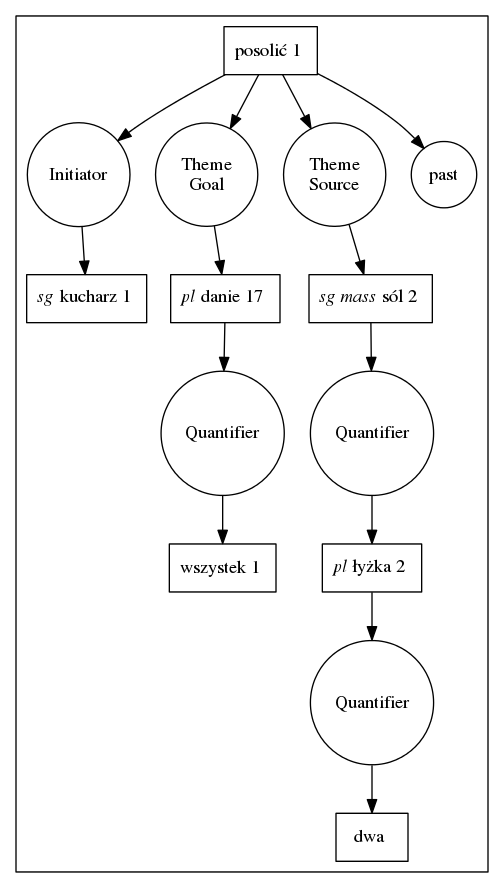
\includegraphics[scale=0.3]{metaopis_sol.png}

%za pierwszym/drugim razem, co drugi raz

\section{Relacja quasi-posiadania i identyczności}
Predykat Poss symbolizuje relację posiadania ({\it piłka chłopca}) oraz pozostałe 
relacje wskazywane przez modyfikator rzeczownikowy w dopełniaczu (przydawkę dopełniaczową)
({\it sposób wykonania}, {\it prezeska organizacji}, {\it obrzeża Warszawy}).
Poss jest domyślną rolą dla przydawki dopełniaczowej. W konkretnych przypadkach np. przy użyciu pojemnikowym jest zastępowana inną relacją.
%W toku dalszych badań Poss zostanie podzielona na podklasy
\[\begin{tikzpicture}
\node[concept] (a) {\sg piłka};
\node[relation, right=1cm of a] (b) {Poss};
\node[concept, right=1cm of b] (c) {\sg chłopiec};
\edge {a} {b};
\edge {b} {c};
\end{tikzpicture}\]

Predykat Poss wykorzystujemy również w sytuacjach, gdy pojęcia mają charakter funkcji biorących odniesienie jednego ze 
swych podrzędników i określających swoje odniesienie na tej podstawie, np odniesieniem frazy 
%{\it pod stołem} będzie miejsce znajdujące się poniżej jakiegoś {\it stołu}.
%Podobnie przy frazie 
{\it kolor piłki} mamy {\it piłkę}, z której wyłuskujemy cechę.
% \[\begin{tikzpicture}
% \node[concept] (a) {pod};
% \node[relation, right=1cm of a] (b) {Poss};
% \node[concept, right=1cm of b] (c) {\sg stół};
% \edge {a} {b};
% \edge {b} {c};
% \end{tikzpicture}\]
\[\begin{tikzpicture}
\node[concept] (a) {\sg kolor};
\node[relation, right=1cm of a] (b) {Poss};
\node[concept, right=1cm of b] (c) {\sg piłka};
\edge {a} {b};
\edge {b} {c};
\end{tikzpicture}\]

% Spójniki podrzędne traktujemy analogicznie jak przyimki, jako 
% operatory, które wyłuskują cechę sytuacji będącej ich argumentem.

Przydawki przyimkowe domyślnie traktujemy tak jak argumenty czasownika.
Na przykład {\it pasta do zębów Jana} jest reprezentowana jako
\[\begin{tikzpicture}
\node[concept] (a) {\sg pasta};
\node[relation, right=1cm of a] (b) {Purp};
\node[concept, below=0.5cm of b] (c) {do};
\node[concept, right=1cm of b] (e) {\pl ząb};
\node[relation, left=1cm of a] (f) {Poss};
\node[concept, left=1cm of f] (g) {\sg osoba ``Jan''};
\edge {a} {b};
\edge [dashed]{b} {c};
\edge {b} {e};
\edge {a} {f};
\edge {f} {g};
\end{tikzpicture}\]
%TODO: można by wprowadzać domyślne zdarzenia/użycia: pasta do [mycia] zębów

Relacja identyczności komunikowana jest przez apozycję oraz przydawkę rzeczoną i zachodzi między odniesieniami obu wyrażeń.
Apozycja (dwa rzeczowniki uzgodnione pod względem przypadka) wyraża dwa określenia tego samego obiektu.
Może to być typ i nazwa, albo dwa różna typy, np. {\it lekarz dentysta} zapiszemy jako
\[\begin{tikzpicture}
\node[concept] (a) {\sg lekarz};
\node[relation, right=1cm of a] (b) {=};
\node[concept, right=1cm of b] (c) {\sg dentysta};
\edge {a} {b};
\edge {b} {c};
\end{tikzpicture}\]
a {\it w mieście Warszawie}, zapiszemy jako 
\[\begin{tikzpicture}
\node[concept] (a) {w};
\node[relation, right=1cm of a] (b) {Loc};
\node[concept, right=1cm of b] (c) {\sg miasto};
\node[relation, right=1cm of c] (d) {=};
\node[concept, right=1cm of d] (e) {\sg ``Warszawa''};
\edge [dashed]{b} {a};
\edge {b} {c};
\edge {c} {d};
\edge {d} {e};
\end{tikzpicture}\]
co możemy skrócić do
\[\begin{tikzpicture}
\node[concept] (a) {w};
\node[relation, right=1cm of a] (b) {Loc};
\node[concept, right=1cm of b] (c) {\sg miasto ``Warszawa''};
\edge [dashed]{b} {a};
\edge {b} {c};
\end{tikzpicture}\]
%{\it artysta malarz}%
Przydawka rzeczowna (wyrażona w mianowniku) nadaje nazwę swojemu nadrzędnikowi, np. {\it na ulicy Ruczaj}, zapiszemy jako 
\[\begin{tikzpicture}
\node[concept] (a) {na};
\node[relation, right=1cm of a] (b) {Loc};
\node[concept, right=1cm of b] (c) {\sg ulica};
\node[relation, right=1cm of c] (d) {=};
\node[concept, right=1cm of d] (e) {\sg ``Ruczaj''};
\edge [dashed]{b} {a};
\edge {b} {c};
\edge {c} {d};
\edge {d} {e};
\end{tikzpicture}\]
\[\begin{tikzpicture}
\node[concept] (a) {na};
\node[relation, right=1cm of a] (b) {Loc};
\node[concept, right=1cm of b] (c) {\sg ulica ``Ruczaj''};
\edge [dashed]{b} {a};
\edge {b} {c};
\end{tikzpicture}\]
%opiekunka pani Gabrysia

Relacja identyczności może zachodzić również pomiędzy podrzędnikami czasownika, 
np. w zdaniu {\it Dionizy pracował jako ogrodnik}. Walentym zjawisko to oznaczone jest rolą Attribute.
\[\begin{tikzpicture}
\node[concept] (a) {pracować};
\node[relation, left=12mm of a] (b) {Init};
\node[concept, below=5mm of b] (c) {\sg osoba ``Dionizy''};
\node[relation, below=5mm of a] (d) {=};
\node[concept, right=1cm of d] (e) {\sg ogrodnik};
\node[relation, left=1cm of c] (f) {Past};
\context{cx}{(a)(b)(c)(d)(e)}{};
\edge {a} {b};
\edge {b} {c};
\edge {c} {d};
\edge {d} {e};
\edge[dashed] {a} {d};
\edge {cx} {f};
\end{tikzpicture}\]
Przerywana strzałka pomiędzy {\it pracować} a relacją ``='' oznacza, że 
relacja identyczności pomiędzy {\it Dionizym} a {\it ogrodnikiem} jest parametryzowana przez zdarzenie {\it pracowania}.

Analogicznie reprezentujemy konstrukcje predykatywne w zdaniach 
{\it Franciszek był studentem}, {\it Każdy stół jest meblem.}
\[\begin{tikzpicture}
\node[concept] (a) {być};
\node[relation, left=15mm of a] (b) {Thme};
\node[concept, below=5mm of b] (c) {\sg osoba ``Franciszek''};
\node[relation, below=5mm of a] (d) {=};
\node[concept, right=1cm of d] (e) {\sg student};
\node[relation, left=1cm of c] (f) {Past};
\context{cx}{(a)(b)(c)(d)(e)}{};
\edge {a} {b};
\edge {b} {c};
\edge {c} {d};
\edge {d} {e};
\edge[dashed] {a} {d};
\edge {cx} {f};
\end{tikzpicture}\]
\[\begin{tikzpicture}
\node[concept] (a) {być};
\node[relation, left=15mm of a] (b) {Thme};
\node[concept, below=5mm of b] (c) {\sg stół};
\node[relation, below=5mm of a] (d) {=};
\node[concept, right=1cm of d] (e) {\sg mebel};
\node[relation, left=10mm of c] (g) {Quant};
\node[concept, left=1cm of g] (h) {każdy};
\node[relation, left=1cm of h] (f) {Pres};
\context{cx}{(a)(b)(c)(d)(e)(h)(g)}{};
\edge {a} {b};
\edge {b} {c};
\edge {c} {d};
\edge {d} {e};
\edge {c} {g};
\edge {g} {h};
\edge[dashed] {a} {d};
\edge {cx} {f};
\end{tikzpicture}\]


% Predykatywne {\it to} możemy zinterpretować tak samo jak {\it być}.
% 
% Dla porównania {\it być} bez predykatywu:
% {\it Stół jest.}
% \[\begin{tikzpicture}
% \node[concept] (a) {być};
% \node[relation, left=1cm of a] (b) {Thme};
% \node[concept, left=1cm of b] (c) {\sg stół};
% \node[relation, right=1cm of a] (d) {Pres};
% \context{cx}{(a)(b)(c)(d)}{};
% \edge {a} {b};
% \edge {b} {c};
% \edge {a} {d};
% \end{tikzpicture}\]

\section{Relacje przestrzenne}
Zazwyczaj wyrażane przez wyrażenia przyimkowe, przysłówki bądź zdania podrzędne.
Przyimki lokatywne reprezentują relacje pomiędzy miejscami.

Relacja Location (Loc) wskazuje położenie sytuacji / zdarzenia.
Relacje Location Source (Loc Src), Location Goal (Loc Goal), Path informują o obecności i kierunku ruchu.
{\it Z Poznania jedzie pociąg przez Warszawę.}:

\[\begin{tikzpicture}
\node[concept] (b) {jechać};
\node[relation, left=25mm of b] (a) {Pres};
\node[relation, right=10mm of b] (c) {Init};
\node[concept, right=10mm of c] (d) {\sg pociąg};
\node[relation, above=5mm of b] (e) {Loc Src};
\node[concept, left=10mm of e] (f) {z};
\node[concept, right=10mm of e] (h) {\sg miasto ''Poznań''};
\node[relation, below=5mm of b] (i) {Path};
\node[concept, left=10mm of i] (j) {przez};
\node[concept, right=10mm of i] (l) {\sg miasto ''Warszawa''};
\context{cx}{(b)(c)(d)(e)(f)(h)(i)(j)(l)}{};
\edge{b}{c};
\edge{cx}{a};
\edge{c}{d};
\edge{b}{e};
\edge[dashed]{e}{f};
\edge{e}{h};
\edge{b}{i};
\edge[dashed]{i}{j};
\edge{i}{l};
\end{tikzpicture}\]

% alternatywna wersja (sensem ``z'' jest ``w''):
% 
% \[\begin{tikzpicture}
% \node[concept] (b) {jechać};
% \node[relation, left=1cm of b] (a) {Pres};
% \node[relation, right=10mm of b] (c) {Init};
% \node[concept, right=10mm of c] (d) {\sg pociąg};
% \node[relation, above=5mm of b] (e) {Loc Src};
% \node[concept, right=10mm of e] (h) {\sg miasto ''Poznań''};
% \node[relation, below=5mm of b] (i) {Path};
% \node[concept, right=10mm of i] (l) {\sg miasto ''Warszawa''};
% \context{f}{(h)}{w}
% \context{j}{(l)}{przez}
% \edge{b}{c};
% \edge{b}{a};
% \edge{c}{d};
% \edge{b}{e};
% \edge{e}{f};
% \edge{b}{i};
% \edge{i}{j};
% \context{cx}{(a)(b)(c)(d)(e)(f)(g)(h)(i)(j)(k)(l)}{};
% \end{tikzpicture}\]
{\it Piłka leży pod stołem.}
\[\begin{tikzpicture}
\node[concept] (a) {leżeć};
\node[relation, left=1cm of a] (b) {Thme};
\node[concept, left=1cm of b] (c) {\sg piłka};
\node[relation, above=0.8cm of a] (d) {Pres};
\node[relation, right=1cm of a] (e) {Loc};
\node[concept, right=1cm of e] (f) {pod};
\node[concept, below=5mm of e] (h) {\sg stół};
\context{cx}{(a)(b)(c)(e)(f)(h)}{};
\edge {a} {b};
\edge {b} {c};
\edge {cx} {d};
\edge {a} {e};
\edge [dashed]{e} {f};
\edge {e} {h};
\end{tikzpicture}\]
{\it Piłka jest pod stołem.}
\[\begin{tikzpicture}
\node[concept] (a) {być};
\node[relation, left=1cm of a] (b) {Thme};
\node[concept, left=1cm of b] (c) {\sg piłka};
\node[relation, above=0.8cm of a] (d) {Pres};
\node[relation, right=1cm of a] (e) {Loc};
\node[concept, right=1cm of e] (f) {pod};
\node[concept, below=5mm of e] (h) {\sg stół};
\context{cx}{(a)(b)(c)(e)(f)(h)}{};
\edge {a} {b};
\edge {b} {c};
\edge {cx} {d};
\edge {a} {e};
\edge [dashed]{e} {f};
\edge {e} {h};
\end{tikzpicture}\]

Przyjmujemy że odpowiadające sobie przyimki lokatywne, ablatywne i adlatywne mają ten sam sens, np {\it pod stołem}, {\it spod stołu}, {\it pod stół}:
\[\begin{tikzpicture}
\node[virtualconcept] (a) {$\cdot$};
\node[relation, right=1cm of a] (b) {Loc};
\node[concept, below=5mm of b] (c) {pod};
\node[concept, right=10mm of b] (e) {\sg stół};
\edge{a}{b};
\edge[dashed]{b}{c};
\edge{b}{e};
\end{tikzpicture}\]
\[\begin{tikzpicture}
\node[virtualconcept] (a) {$\cdot$};
\node[relation, right=1cm of a] (b) {Loc Src};
\node[concept, below=5mm of b] (c) {pod};
\node[concept, right=10mm of b] (e) {\sg stół};
\edge{a}{b};
\edge[dashed]{b}{c};
\edge{b}{e};
\end{tikzpicture}\]
\[\begin{tikzpicture}
\node[virtualconcept] (a) {$\cdot$};
\node[relation, right=1cm of a] (b) {Loc Goal};
\node[concept, below=5mm of b] (c) {pod};
\node[concept, right=10mm of b] (e) {\sg stół};
\edge{a}{b};
\edge[dashed]{b}{c};
\edge{b}{e};
\end{tikzpicture}\]

W niektórych sytuacjach argument przyimka opisującego relację przestrzenną nie jest jawny i staje się on przysłówkiem
z argumentem okazjonalnym bądź koreferencyjnym, np:
{\it Mieszkam nieopodal fontanny} vs {\it Mieszkam nieopodal}.
\[\begin{tikzpicture}
\node[concept] (t) {mieszkać};
\node[relation, left=1cm of t] (ts) {Init};
\node[concept, left=1cm of ts] (s) {\sg \ind ja};
\node[relation, above=0.8cm of t] (pr) {Pres};
\node[relation, right=1cm of t] (tk) {Loc};
\node[concept, below=5mm of tk] (k) {nieopodal};
\node[concept, right=1cm of tk] (l) {\sg fontanna};
\context{cx}{(t)(ts)(s)(tk)(k)(l)}{};
\edge {t} {ts};
\edge {cx} {pr};
\edge {ts} {s};
\edge {t} {tk};
\edge [dashed]{tk} {k};
\edge {tk} {l};
\end{tikzpicture}\]
\[\begin{tikzpicture}
\node[concept] (t) {mieszkać};
\node[relation, left=1cm of t] (ts) {Init};
\node[concept, left=1cm of ts] (s) {\sg \ind ja};
\node[relation, above=0.8cm of t] (pr) {Pres};
\node[relation, right=1cm of t] (tk) {Loc};
\node[concept, below=5mm of tk] (k) {nieopodal};
\node[concept, right=1cm of tk] (l) {\ind pro};
\context{cx}{(t)(ts)(s)(tk)(k)(l)}{};
\edge {t} {ts};
\edge {cx} {pr};
\edge {ts} {s};
\edge {t} {tk};
\edge [dashed]{tk} {k};
\edge {tk} {l};
\end{tikzpicture}\]
Przyjmujemy, że sens leksemu {\it nieopodal} jest identyczny w obu wypadkach.
Podobnie zachowują się: {\it obok, blisko, dookoła, naokoło, naprzeciw, opodal, wewnątrz, wokół, wzdłuż}.

Wieloargumentowy przyimek {\it między} traktujemy jak przyimek jednoargumentowy,
którego podrzędnikiem jest koordynacja, np. {\it między stołem, krzesłem a pianinem}
\[\begin{tikzpicture}
\node[concept] (a) {\sg stół};
\node[concept, right=5mm of a] (b) {\sg krzesło};
\node[concept, right=5mm of b] (c) {\sg pianino};
\context{v}{(a)(b)(c)}{a};
\node[relation, right=10mm of c] (d) {Loc};
\node[concept, right=10mm of d] (e) {między};
\edge{d}{v};
\edge[dashed]{d}{e};
\end{tikzpicture}\]
{\it między fotelami}
\[\begin{tikzpicture}
\node[concept] (a) {\pl fotel};
\node[relation, right=10mm of a] (d) {Loc};
\node[concept, right=10mm of d] (e) {między};
\edge{d}{a};
\edge[dashed]{d}{e};
\end{tikzpicture}\]
%{\it Kot jest między stołem a fotelem}
%{\it Kot jest między fotelami}

Przyimki lokatywne mogą być modyfikowane, np. {\it dość głęboko w szafie},
{\it 5 km od domu}, {\it po lewej (prawej, drugiej) stronie lustra}.
%TODO: czy tu na pewno powinna być relacja Manner
\[\begin{tikzpicture}
\node[concept] (t) {w};
\node[relation, left=1cm of t] (ts) {Loc};
\node[concept, left=1cm of ts] (s) {\sg szafa};
\node[relation, right=1cm of t] (a) {Manr};
\node[concept, right=1cm of a] (b) {głęboko};
\node[relation, right=1cm of b] (c) {Manr};
\node[concept, right=1cm of c] (d) {dość};
\edge [dashed]{ts} {t};
\edge {ts} {s};
\edge {t} {a};
\edge {a} {b};
\edge {b} {c};
\edge {c} {d};
\end{tikzpicture}\]
\[\begin{tikzpicture}
\node[concept] (t) {od};
\node[relation, left=1cm of t] (ts) {Loc};
\node[concept, left=1cm of ts] (s) {\sg dom};
\node[relation, right=1cm of t] (a) {Manr};
\node[concept, right=1cm of a] (b) {kilometr};
\node[relation, right=1cm of b] (c) {Count};
\node[concept, right=1cm of c] (d) {5};
\edge [dashed]{ts} {t};
\edge {ts} {s};
\edge {t} {a};
\edge {a} {b};
\edge {b} {c};
\edge {c} {d};
\end{tikzpicture}\]
\[\begin{tikzpicture}
\node[concept] (t) {po stronie};
\node[relation, left=1cm of t] (ts) {Loc};
\node[concept, left=1cm of ts] (s) {\sg lustro};
\node[relation, right=1cm of t] (a) {Manr};
\node[concept, right=1cm of a] (b) {lewy};
\edge [dashed]{ts} {t};
\edge {ts} {s};
\edge {t} {a};
\edge {a} {b};
\end{tikzpicture}\]
%w szczególnym związku z - zmodyfikowany przyimek złożony
Przyimki mogą być też modyfikowane nieintersektywnie np. {\it prawie na rogu ulicy}
\[\begin{tikzpicture}
\node[concept] (t) {prawie(na rogu)};
\node[relation, left=1cm of t] (ts) {Loc};
\node[concept, left=1cm of ts] (s) {\sg ulica};
\edge [dashed]{ts} {t};
\edge {ts} {s};
\end{tikzpicture}\]

\section{Sytuacje, procesy i relacje czasowe}
Każdy proces wymieniowy w zdaniu umieszczamy w osobnym kontekście sytuacyjnym. 
% Nawet jeśli procesy są wyrażone imiesłowem przysłówkowym uprzednim lub imiesłowem przymiotnikowym czynnym, 
% który stwierdza równoczesność zdarzeń mogą mieć inny czas rozpoczęcia i zakończenia.
W kontekstach sytuacyjnych uczestnicy istnieją a relacje między nimi 
zachodzą przez cały czas trwania sytuacji, chyba że uczestnik jest 
połączony relacją z procesem. W takiej sytuacji może on zostać
w trakcie procesu stworzony, czyli zaistnieć dopiero na jego 
końcu, może powstawać stopniowo, może też przestać istnieć.
Z kolei relacje wychodzące z procesów mogą się zmieniać w trakcie procesu.
Natomiast relacje czasowe przypisane zdarzeniu dotyczą każdego uczestnika sytuacji a 
czas zdarzenia przysługuje całej sytuacji. 

Na potrzeby reprezentacji za pomocą grafów semantycznych
przyjmujemy, że relacje czasowe wiążą czas z sytuacjami,
a znajdujące się w kontekstach pojęcia i relacje uznamy za fluenty 
niejawnie przez ten czas parametryzowane.

Relacje czasowe zazwyczaj wyrażane przez wyrażenia przyimkowe, przysłówki bądź zdania podrzędne.
Przyimki temporalne reprezentują relacje pomiędzy punktami w czasie, interwałami oraz ich zbiorami.
Relacje Time i Duration (Dur) informują o czasie, przypisanym do danego obiektu (zazwyczaj zdarzenia) oraz czasie jego trwania.

Spójnik {\it gdy} w jednym ze swoich znaczeń bierze sytuację (zdarzenie) i generuje jej czas, np. {\it Wszedł, gdy go wpuścili}:
\[\begin{tikzpicture}
\node[concept] (a) {wejść};
\node[relation, left=1cm of a] (b) {Init};
\node[concept, left=1cm of b] (c) {\corf pro-on};
\node[relation, right=1cm of a] (d) {Past};
\node[relation, below=0.5cm of a] (e) {Time};
\node[concept, right=1cm of e] (f) {gdy};
\context{cx}{(a)(b)(c)}{};
\node[concept, below=2.2cm of a] (h) {wpuścić};
\node[relation, left=1cm of h] (i) {Init};
\node[concept, left=1cm of i] (j) {\deict pro-oni};
\node[relation, below=0.8cm of h] (k) {Past};
\node[relation, right=1cm of h] (l) {Thme};
\node[concept, right=1cm of l] (m) {\corf on};
\context{cy}{(h)(i)(j)(l)(m)}{};
\edge {a} {b};
\edge {b} {c};
\edge {cx} {d};
\edge {cx} {e};
\edge [dashed]{e} {f};
\edge {e} {cy};
\edge {h} {i};
\edge {i} {j};
\edge {cy} {k};
\edge {h} {l};
\edge {l} {m};
\end{tikzpicture}\]

Przyimek {\it po} w znaczeniu czasowym odwołuje się do wcześniejszej sytuacji, bądź wcześniejszego zdarzenia.
Może być ono wyrażone przez odsłownik, bądź rzeczownik, np:
{\it Po powrocie z zagranicy Sebastian pracował w fabryce}, {\it Po ukończeniu studiów Sebastian pracował na poczcie.}
% \[\begin{tikzpicture}
% \node[concept] (a) {pracować};
% \node[relation, left=1cm of a] (b) {Init};
% \node[concept, left=1cm of b] (c) {\sg osoba ``Sebastian''};
% \node[relation, above=0.5cm of b] (d) {Past};
% \node[relation, right=1cm of a] (e) {Time};
% \node[concept, right=1cm of e] (f) {po};
% \node[relation, right=1cm of f] (g) {Poss};
% \node[relation, right=1cm of d] (l) {Loc};
% \node[concept, right=1cm of l] (m) {w};
% \node[relation, right=1cm of m] (n) {Poss};
% \node[concept, right=1cm of n] (o) {\sg fabryka};
% \node[concept, below=1cm of c] (h) {powrót};
% \node[relation, right=1cm of h] (p) {Loc Src};
% \node[concept, right=1cm of p] (q) {z};
% \node[relation, right=1cm of q] (i) {Poss};
% \node[concept, right=1cm of i] (j) {\sg zagranica};
% \context{cy}{(h)(i)(j)(p)(q)}{};
% \context{cx}{(a)(b)(c)(d)(e)(f)(g)(cy)}{};
% \edge {a} {b};
% \edge {b} {c};
% \edge {a} {d};
% \edge {a} {e};
% \edge {e} {f};
% \edge {f} {g};
% \edge {g} {cy};
% \edge {q} {i};
% \edge {i} {j};
% \edge {a} {l};
% \edge {l} {m};
% \edge {m} {n};
% \edge {n} {o};
% \edge {h} {p};
% \edge {p} {q};
% \end{tikzpicture}\]

\[\begin{tikzpicture}
\node[concept] (a) {pracować};
\node[relation, left=1cm of a] (b) {Init};
\node[concept, left=1cm of b] (c) {\sg osoba ``Sebastian''};
\node[relation, below=1.6cm of c] (d) {Past};
\node[relation, below=1.6cm of b] (e) {Time};
\node[concept, right=1cm of e] (f) {po};
\node[relation, right=1cm of a] (l) {Loc};
\node[concept, right=1cm of l] (m) {w};
\node[concept, below=5mm of l] (o) {\sg fabryka};
\node[concept, below=3.5cm of c] (h) {powrót};
\node[relation, right=1cm of h] (p) {Loc Src};
\node[concept, right=1cm of p] (q) {z};
\node[concept, below=5mm of p] (j) {\sg zagranica};
\context{cx}{(a)(b)(c)(m)(o)}{};
\context{cy}{(h)(j)(p)(q)}{};
\edge {a} {b};
\edge {b} {c};
\edge {cx} {d};
\edge {cx} {e};
\edge [dashed]{e} {f};
\edge {e} {cy};
\edge {p} {j};
\edge {a} {l};
\edge [dashed]{l} {m};
\edge {l} {o};
\edge {h} {p};
\edge [dashed]{p} {q};
\end{tikzpicture}\]

% \[\begin{tikzpicture}
% \node[concept] (a) {pracować};
% \node[relation, left=1cm of a] (b) {Init};
% \node[concept, left=1cm of b] (c) {\sg osoba ``Sebastian''};
% \node[relation, above=0.5cm of b] (d) {Past};
% \node[relation, right=1cm of a] (e) {Time};
% \node[concept, right=1cm of e] (f) {po};
% \node[relation, right=1cm of f] (g) {Poss};
% \node[relation, right=1cm of d] (l) {Loc};
% \node[concept, right=1cm of l] (m) {na};
% \node[relation, right=1cm of m] (n) {Poss};
% \node[concept, right=1cm of n] (o) {\sg poczta};
% \node[concept, below=1cm of a] (h) {ukończyć};
% \node[relation, left=1cm of h] (i) {Init};
% \node[concept, left=1cm of i] (j) {\sg {\it ter} \corf pro};
% \node[relation, below=0.5cm of h] (k) {Past};
% \node[relation, right=1cm of h] (p) {Thme};
% \node[concept, right=1cm of p] (q) {studia};
% \context{cy}{(h)(i)(j)(k)(p)(q)}{};
% \context{cx}{(a)(b)(c)(d)(e)(f)(g)(cy)}{};
% \edge {a} {b};
% \edge {b} {c};
% \edge {a} {d};
% \edge {a} {e};
% \edge {e} {f};
% \edge {f} {g};
% \edge {g} {cy};
% \edge {h} {i};
% \edge {i} {j};
% \edge {h} {k};
% \edge {a} {l};
% \edge {l} {m};
% \edge {m} {n};
% \edge {n} {o};
% \edge {h} {p};
% \edge {p} {q};
% \end{tikzpicture}\]

\[\begin{tikzpicture}
\node[concept] (a) {pracować};
\node[relation, left=1cm of a] (b) {Init};
\node[concept, left=1cm of b] (c) {\sg osoba ``Sebastian''};
\node[relation, below=1.6cm of c] (d) {Past};
\node[relation, below=1.6cm of b] (e) {Time};
\node[concept, right=1cm of e] (f) {po};
\node[relation, right=1cm of a] (l) {Loc};
\node[concept, right=1cm of l] (m) {na};
\node[concept, below=5mm of l] (o) {\sg poczta};
\node[concept, below=1cm of f] (h) {ukończyć};
\node[relation, left=1cm of h] (i) {Init};
\node[concept, left=1cm of i] (j) {\corf pro};
\node[relation, below=0.8cm of h] (k) {Past};
\node[relation, right=1cm of h] (p) {Thme};
\node[concept, right=1cm of p] (q) {studia};
\context{cx}{(a)(b)(c)(m)(o)}{};
\context{cy}{(h)(i)(j)(p)(q)}{};
\edge {a} {b};
\edge {b} {c};
\edge {cx} {d};
\edge {cx} {e};
\edge [dashed]{e} {f};
\edge {e} {cy};
\edge {h} {i};
\edge {i} {j};
\edge {cy} {k};
\edge {a} {l};
\edge [dashed]{l} {m};
\edge {l} {o};
\edge {h} {p};
\edge {p} {q};
\end{tikzpicture}\]

% Jest to też powód dla którego każdy proces wymieniowy w zdaniu powienien być
% umieszczony w osobnym kontekście sytuacyjnym. 
% Nawet jeśli procesy są wyrażone imiesłowem przysłówkowym uprzednim lub imiesłowem przymiotnikowym czynnym, 
% który stwierdza równoczesność zdarzeń mogą mieć inny czas rozpoczęcia i zakończenia.

{\it Słoń biegnie trąbiąc.} 
\[\begin{tikzpicture}
\node[concept] (a) {biec};
\node[relation, left=1cm of a] (b) {Init};
\node[concept, left=1cm of b] (c) {\sg słoń $\ast x$};
\node[relation, right=1cm of a] (d) {Pres};
\node[relation, below=0.5cm of a] (e) {Time};
\node[concept, right=1cm of e] (f) {czas};
\node[concept, below=1cm of e] (h) {trąbić};
\node[relation, left=1cm of h] (i) {Init};
\node[concept, left=1cm of i] (j) {T $?x$};
\node[relation, right=1cm of h] (g) {Time};
\context{cx}{(a)(b)(c)}{};
\context{cy}{(h)(i)(j)}{};
\edge {a} {b};
\edge {b} {c};
\edge {cx} {d};
\edge {cx} {e};
\edge {e} {f};
\edge {g} {f};
\edge {cy} {g};
\edge {h} {i};
\edge {i} {j};
\end{tikzpicture}\]
Symbol $\ast x$ wprowadza zmienną $x$, która oznacza odniesienie pojęcia słoń, 
a symbol $?x$ oznacza użycie zmiennej $x$. Razem wyrażają koreferencję.
Pudełko {\it czas} służy do zareprezentowania równoczesności obu zdarzeń.

{\it Trąbiący słoń biegnie.}
\[\begin{tikzpicture}
\node[concept] (a) {biec};
\node[relation, left=1cm of a] (b) {Init};
\node[concept, left=1cm of b] (c) {\sg słoń $\ast x$};
\node[relation, right=1cm of a] (d) {Pres};
\node[relation, below=0.5cm of a] (e) {Time};
\node[concept, right=1cm of e] (f) {czas};
\node[concept, below=1cm of e] (h) {trąbić};
\node[relation, left=1cm of h] (i) {Init};
\node[concept, left=1cm of i] (j) {T $?x$};
\node[relation, right=1cm of h] (g) {Time};
\context{cx}{(a)(b)(c)}{};
\context{cy}{(h)(i)(j)}{};
\edge {a} {b};
\edge {b} {c};
\edge {cx} {d};
\edge {cx} {e};
\edge {e} {f};
\edge {g} {f};
\edge {cy} {g};
\edge {h} {i};
\edge {i} {j};
\end{tikzpicture}\]

Następstwo zdarzeń reprezentujemy za pomocą relacji Succ, np {\it Słoń odpoczywa zatrąbiwszy.}
\[\begin{tikzpicture}
\node[concept] (a) {odpoczywać};
\node[relation, left=1cm of a] (b) {Init};
\node[concept, left=1cm of b] (c) {\sg słoń};
\node[relation, right=1cm of a] (d) {Pres};
\node[relation, left=1cm of c] (e) {Succ};
\node[concept, below=1cm of a] (h) {zatrąbić};
\node[relation, left=1cm of h] (i) {Init};
\node[concept, left=1cm of i] (j) {$\corf$ pro};
\context{cx}{(a)(b)(c)}{};
\context{cy}{(h)(i)(j)}{};
\edge {a} {b};
\edge {b} {c};
\edge {cx} {d};
\edge {cy} {e};
\edge {e} {cx};
\edge {h} {i};
\edge {i} {j};
\end{tikzpicture}\]
% \[\begin{tikzpicture}
% \node[concept] (a) {odpoczywać};
% \node[relation, left=1cm of a] (b) {Init};
% \node[concept, left=1cm of b] (c) {\sg słoń $\ast x$};
% \node[relation, right=1cm of a] (d) {Pres};
% \node[relation, below=0.5cm of a] (e) {Succ};
% \node[concept, below=1cm of e] (h) {zatrąbić};
% \node[relation, left=1cm of h] (i) {Init};
% \node[concept, left=1cm of i] (j) {T $?x$};
% \context{cx}{(a)(b)(c)}{};
% \context{cy}{(h)(i)(j)}{};
% \edge {a} {b};
% \edge {b} {c};
% \edge {cx} {d};
% \edge {cx} {e};
% \edge {e} {cy};
% \edge {h} {i};
% \edge {i} {j};
% \end{tikzpicture}\]

{\it Kupiłem ręcznie malowaną filiżankę.}
\[\begin{tikzpicture}
\node[concept] (a) {kupić};
\node[relation, left=1cm of a] (b) {Init};
\node[concept, left=1cm of b] (c) {\ind pro-ja-m};
\node[relation, above=0.8cm of a] (d) {Past};
\node[relation, right=1cm of a] (e) {Thme};
\node[concept, right=1cm of e] (f) {\sg filiżanka $\ast x$};
\node[concept, below=3cm of a] (h) {malować};
\node[relation, left=1cm of h] (i) {Manner};
\node[concept, left=1cm of i] (j) {ręcznie};
\node[relation, right=1cm of h] (g) {Thme};
\node[concept, right=1cm of g] (k) {T $?x$};
\context{cx}{(a)(b)(c)(e)(f)}{};
\context{cy}{(h)(i)(j)(g)(k)}{};
\node[relation, below=0.8cm of b] (p) {Succ};
\edge {a} {b};
\edge {b} {c};
\edge {cx} {d};
\edge {a} {e};
\edge {e} {f};
\edge {g} {k};
\edge {h} {g};
\edge {h} {i};
\edge {i} {j};
\edge {p} {cx};
\edge {cy} {p};
\end{tikzpicture}\]

Czasowniki {\it być} i {\it zostać} w stronie biernej
traktujemy jako czasowniki posiłkowe wnoszące do semantyki jedynie czas, np
{\it Filiżanka jest malowana ręcznie.}
% \[\begin{tikzpicture}
% \node[concept] (a) {być};
% \node[relation, left=1cm of a] (d) {Pres};
% \node[relation, right=1cm of a] (e) {Thme};
% \node[concept, right=1cm of e] (f) {\sg filiżanka $\ast x$};
% \node[concept, below=1.2cm of a] (h) {malować};
% \node[relation, left=1cm of h] (i) {Manner};
% \node[concept, left=1cm of i] (j) {ręcznie};
% \node[relation, right=1cm of h] (g) {Thme};
% \node[concept, right=1cm of g] (k) {T $?x$};
% \context{cy}{(h)(i)(j)(g)(k)}{};
% \context{cx}{(a)(d)(e)(f)}{};
% \edge {a} {d};
% \edge {a} {e};
% \edge {e} {f};
% \edge {g} {k};
% \edge {h} {g};
% \edge {h} {i};
% \edge {i} {j};
% \end{tikzpicture}\]
% W powyższym zdaniu kontekst z {\it być} można uznać za redundantny,
% ale pozostanie by reprezentacja strony biernej nie różniła się od innych
% użyć predykatynwych.
% albo
\[\begin{tikzpicture}
\node[concept] (h) {malować};
\node[relation, left=1cm of h] (i) {Manner};
\node[concept, left=1cm of i] (j) {ręcznie};
\node[relation, right=1cm of h] (g) {Thme};
\node[concept, right=1cm of g] (k) {\sg filiżanka};
\node[relation, left=1cm of j] (d) {Pres};
\context{cy}{(h)(i)(j)(g)(k)}{};
\edge {g} {k};
\edge {h} {g};
\edge {h} {i};
\edge {i} {j};
\edge {cy} {d};
\end{tikzpicture}\]

{\it Filiżanka została pomalowana ręcznie.}
% \[\begin{tikzpicture}
% \node[concept] (a) {zostać};
% \node[relation, left=1cm of a] (d) {Past};
% \node[relation, right=1cm of a] (e) {Thme};
% \node[concept, right=1cm of e] (f) {\sg filiżanka $\ast x$};
% \node[concept, below=1.2cm of a] (h) {pomalować};
% \node[relation, left=1cm of h] (i) {Manner};
% \node[concept, left=1cm of i] (j) {ręcznie};
% \node[relation, right=1cm of h] (g) {Thme};
% \node[concept, right=1cm of g] (k) {T $?x$};
% \context{cy}{(h)(i)(j)(g)(k)}{};
% \context{cx}{(a)(d)(e)(f)}{};
% \edge {a} {d};
% \edge {a} {e};
% \edge {e} {f};
% \edge {g} {k};
% \edge {h} {g};
% \edge {h} {i};
% \edge {i} {j};
% \end{tikzpicture}\]
% albo
\[\begin{tikzpicture}
\node[concept] (h) {pomalować};
\node[relation, left=1cm of h] (i) {Manner};
\node[concept, left=1cm of i] (j) {ręcznie};
\node[relation, right=1cm of h] (g) {Thme};
\node[concept, right=1cm of g] (k) {\sg filiżanka};
\node[relation, left=1cm of j] (d) {Past};
\context{cy}{(h)(i)(j)(g)(k)}{};
\edge {g} {k};
\edge {h} {g};
\edge {h} {i};
\edge {i} {j};
\edge {cy} {d};
\end{tikzpicture}\]

% TODO co zrobić z {\it Twarz Eduarda stała się napięta}

Leksem {\it ledwo} użyty w znaczeniu czasowym funktor biorący zdarzenie i generujący czas chwilę po nim. W funkcji 
spójnika podrzędnego, czas ten określa czas zdarzenia ze zdania nadrzędnego, w funkcji przysłówka 
czas ten określa czas zdarzenia wynikającego z kontekstu. %, co można wyrazić jako pro-zdarzenie.
Np.: {\it Słońce ledwo wzeszło}, {\it Ledwo zabrał się do pracy, zadzwonił telefon}:
\[\begin{tikzpicture}
\node[concept] (a) {wzejść};
\node[relation, left=1cm of a] (b) {Init};
\node[concept, left=1cm of b] (c) {\sg słońce};
\node[relation, above=0.8cm of a] (d) {Past};
\context{cx}{(a)(b)(c)}{};
\node[relation, below=0.8cm of b] (p) {Time};
\node[concept, right=1cm of p] (q) {\ind ledwo};
\edge {a} {b};
\edge {b} {c};
\edge {cx} {d};
\edge {cx} {p};
\edge {p} {q};
\end{tikzpicture}\]
\[\begin{tikzpicture}
\node[concept] (a) {zabrać się};
\node[relation, left=1cm of a] (b) {Init};
\node[concept, left=1cm of b] (c) {\deict pro-on};
\node[relation, below=0.8cm of c] (d) {Past};
\node[relation, right=1cm of a] (e) {Thme};
\node[concept, right=1cm of e] (f) {\sg praca};
\node[concept, below=2.8cm of a] (h) {zadzwonić};
\node[relation, right=1cm of h] (g) {Thme};
\node[concept, right=1cm of g] (k) {\sg telefon};
\context{cx}{(a)(b)(c)(e)(f)}{};
\context{cy}{(h)(g)(k)}{};
\node[relation, right=1cm of q] (r) {Time};
\node[concept, left=1cm of r] (q) {ledwo};
\node[relation, left=1cm of h] (l) {Past};
\edge {a} {b};
\edge {b} {c};
\edge {cx} {d};
\edge {a} {e};
\edge {e} {f};
\edge {g} {k};
\edge {h} {g};
\edge {r} {cx};
\edge {cy} {r};
\edge [dashed]{r} {q};
\edge {cy} {l};
\end{tikzpicture}\]

{\it Jan przybył na dwie umówione przez Marysię kolacje.}
\[\begin{tikzpicture}
\node[concept] (a) {przybyć};
\node[relation, left=1cm of a] (b) {Init};
\node[concept, left=1cm of b] (c) {\sg osoba ``Jan''};
\node[relation, below=0.8cm of c] (d) {Past};
\node[relation, right=1cm of a] (e) {Thme};
\node[concept, right=1cm of e] (f) {kolacja $\ast x$};
\node[relation, right=1cm of f] (g) {Count};
\node[concept, right=1cm of g] (h) {2};
\node[relation, below=1cm of a] (r) {Succ};
\node[concept, below=2.8cm of a] (i) {umówić};
\node[relation, right=1cm of i] (j) {Thme};
\node[concept, right=1cm of j] (k) {T $?x$};
\node[relation, left=1cm of i] (l) {Init};
\node[concept, left=1cm of l] (m) {\sg osoba ``Marysia''};
\context{cx}{(a)(b)(c)(e)(f)(g)(h)}{};
\context{cy}{(i)(j)(k)(l)(m)}{};
\edge {a} {b};
\edge {b} {c};
\edge {cx} {d};
\edge {a} {e};
\edge {e} {f};
\edge {f} {g};
\edge {g} {h};
\edge {r} {cx};
\edge {cy} {r};
\edge {i} {j};
\edge {j} {k};
\edge {i} {l};
\edge {l} {m};
\end{tikzpicture}\]

Poszczególne symbole czasowe (numery lat, dni tygodnia, numery godzin, minut, itp.) traktujemy 
jako nazwy interwałów. Wiele interwałów może nosić tą samą nazwę (np. co tydzień jest {\it poniedziałek})
podobnie jak wiele osób może mieć to samo imię, czy nazwisko.
Złożone określenia czasu --- 16 grudnia 2016 --- traktujemy interwał odpowiadający dniowi o nazwie 16.
Dzień ten jest dookreślony przez przynależność do miesiąca grudnia, który z kolei określony 
przynależnością do roku o numerze 2016. Zatem zdanie {\it Urodził się 16 grudnia 2016} będzie miało interpretację
\[\begin{tikzpicture}
\node[concept] (a) {urodzić się};
\node[relation, left=1cm of a] (b) {Thme};
\node[concept, left=1cm of b] (c) {\deict pro-on};
\node[relation, right=1cm of a] (d) {Past};
\context{cx}{(a)(b)(c)}{};
\node[relation, below=0.8cm of c] (e) {Time};
\node[concept, right=1cm of e] (f) {\sg dzień ``16''};
\node[relation, right=1cm of f] (g) {Poss};%TODO relacja
\node[concept, right=1cm of g] (h) {\sg miesiąc ``grudzień''};
\node[relation, right=1cm of h] (i) {Poss};%TODO relacja
\node[concept, right=1cm of i] (j) {\sg rok ``2016''};
\edge {a} {b};
\edge {b} {c};
\edge {cx} {d};
\edge {cx} {e};
\edge {e} {f};
\edge {f} {g};
\edge {g} {h};
\edge {h} {i};
\edge {i} {j};
\end{tikzpicture}\]
{\it Padało do wtorku.}
\[\begin{tikzpicture}
\node[concept] (a) {padać};
\node[relation, left=1cm of a] (b) {Thme};
\node[concept, left=1cm of b] (c) {\deict pro-ono};%TODO czy tu jest pro???
\node[relation, right=1cm of a] (d) {Past};
\context{cx}{(a)(b)(c)}{};
\node[relation, below=0.8cm of c] (e) {Time};
\node[concept, left=1cm of e] (f) {do};
\node[concept, right=1cm of e] (h) {\sg dzień tygodnia ``wtorek''};
\edge {a} {b};
\edge {b} {c};
\edge {cx} {d};
\edge {cx} {e};
\edge [dashed]{e} {f};
\edge {e} {h};
\end{tikzpicture}\]
{\it Obudził się o 12:21.}
\[\begin{tikzpicture}
\node[concept] (a) {obudzić się};
\node[relation, left=1cm of a] (b) {Expr};
\node[concept, left=1cm of b] (c) {\deict pro-on};
\node[relation, right=1cm of a] (d) {Past};
\context{cx}{(a)(b)(c)}{};
\node[relation, below=0.8cm of c] (e) {Time};
\node[concept, left=1cm of e] (f) {o};
\node[concept, right=1cm of e] (h) {\sg godzina ``12''};
\node[relation, right=1cm of h] (i) {Poss};%TODO relacja
\node[concept, right=1cm of i] (j) {\sg minuta ``21''};
\edge {a} {b};
\edge {b} {c};
\edge {cx} {d};
\edge {cx} {e};
\edge [dashed]{e} {f};
\edge {e} {h};
\edge {h} {i};
\edge {i} {j};
\end{tikzpicture}\]
{\it Przyjdzie rano.}
\[\begin{tikzpicture}
\node[concept] (a) {przyjść};
\node[relation, left=1cm of a] (b) {Init};
\node[concept, left=1cm of b] (c) {\deict pro-3sg};
\node[relation, right=1cm of a] (d) {Fut};
\context{cx}{(a)(b)(c)}{};
\node[relation, below=0.8cm of c] (e) {Time};
\node[concept, right=1cm of e] (f) {rano};
\edge {a} {b};
\edge {b} {c};
\edge {cx} {d};
\edge {cx} {e};
\edge {e} {f};
\end{tikzpicture}\]
{\it Śnieg stopniał wiosną.}
\[\begin{tikzpicture}
\node[concept] (a) {stopnieć};
\node[relation, left=1cm of a] (b) {Thme};
\node[concept, left=1cm of b] (c) {\sg śnieg};
\node[relation, right=1cm of a] (d) {Past};
\context{cx}{(a)(b)(c)}{};
\node[relation, below=0.8cm of c] (e) {Time};
\node[concept, right=1cm of e] (f) {\sg wiosna};
\edge {a} {b};
\edge {b} {c};
\edge {cx} {d};
\edge {cx} {e};
\edge {e} {f};
\end{tikzpicture}\]
{\it Ptak przebywał w Nigerii przez zimę}
\[\begin{tikzpicture}
\node[concept] (a) {przebywać};
\node[relation, left=1cm of a] (b) {Init};
\node[concept, left=1cm of b] (c) {\sg ptak};
\node[relation, below=1.8cm of b] (d) {Past};
\node[relation, right=1cm of a] (e) {Loc};
\node[concept, right=1cm of e] (f) {w};
\node[concept, below=5mm of e] (j) {\sg kraj ``Nigeria''};
\context{cx}{(a)(b)(c)(e)(f)(j)}{};
\node[relation, below=1.8cm of e] (p) {Dur};
\node[concept, left=1cm of p] (q) {przez};
\node[concept, right=1cm of p] (s) {\sg zima};
\edge {a} {b};
\edge {b} {c};
\edge {cx} {d};
\edge {a} {e};
\edge [dashed]{e} {f};
\edge {e} {j};
\edge {cx} {p};
\edge [dashed]{p} {q};
\edge {p} {s};
\end{tikzpicture}\]
%TODO: umowa z dnia 7 grudnia 2016


%TODO
% Każdy rzeczownik pospolity pełniący funkcję podmiotu może wprowadzać 
% informację o czasie, kiedy można go orzec o jego odniesieniu, a każda nazwa własna
% - o czasie kiedy przysauguje swojemu odniesieniu. Dzięki temu formuła, którą
% podmiot wprowadza do reprezentacji zdania, nie musi być prawdziwa wtedy,
% gdy prawdziwe jest orzeczenie, co czyni zadość obserwacjom językowym, np.
% Dyrektorka też zdawała maturę.
\section{Cechy}

Zazwyczaj cechy (atrybuty) wyrażane są przez przymiotniki, przysłówki lub wyrażenia przyimkowe, np.: {\it Intensywnie różowy słoń trąbi}: 
\[\begin{tikzpicture}
\node[concept] (t) {trąbić};
\node[relation, right=1cm of t] (ts) {Init};
\node[concept, right=1cm of ts] (s) {\sg słoń};
\node[relation, left=1cm of t] (pr) {Pres};
\node[relation, right=1cm of s] (sk) {Attr};
\node[concept, right=1cm of sk] (k) {różowy};
\node[relation, right=1cm of k] (kl) {Manr};
\node[concept, right=1cm of kl] (l) {intensywnie};
\context{cx}{(t)(ts)(s)(sk)(k)(kl)(l)}{};
\edge {t} {ts};
\edge {cx} {pr};
\edge {ts} {s};
\edge {s} {sk};
\edge {sk} {k};
\edge {k} {kl};
\edge {kl} {l};
\end{tikzpicture}\]

Cechę opisywaną przez przymiotnik domyślnie wyrażamy rolą Attribute (Attr)
zaś cechę opisywaną przez przysłówek wyrażamy rolą Manner (Manr).

W przypadku wyrażeń przyimkowych opisujących cechy rzeczowników również stosujemy rolę Attr,
np.: {\it książka na temat grzybów}, {\it książka o grzybach}:
\[\begin{tikzpicture}
\node[concept] (a) {\sg książka};
\node[relation, right=1cm of a] (b) {Attr};
\node[concept, right=1cm of b] (c) {na temat};
\node[concept, below=5mm of b] (e) {\pl grzyb};
\edge {a} {b};
\edge [dashed]{b} {c};
\edge {b} {e};
\end{tikzpicture}\]
\[\begin{tikzpicture}
\node[concept] (a) {\sg książka};
\node[relation, right=1cm of a] (b) {Attr};
\node[concept, right=1cm of b] (c) {o};
\node[concept, below=5mm of b] (e) {\pl grzyb};
\edge {a} {b};
\edge [dashed]{b} {c};
\edge {b} {e};
\end{tikzpicture}\]
{\it na temat} jest przyimkiem złożonym traktowanym jako pojedyncza jednostka leksykalna,
natomiast {\it o} w znaczeniu użytym w powyższym przykładzie jest jego synonimem.
Przyimki złożone wskazują w swojej treści nazwę cechy, której dotyczą.

%TODO: jak to jest dla czasowników


Cechy danego przedmiotu mogą być składniowo wyrażone przez podrzędnik czasownika.
Słownik walencyjny Walenty sygnalizuje takie sytuacje nadając podrzędnikowi
wyrażającemu cechę rolę Attribute oraz czyniąc go kontrolowanym przez 
podrzędnik będący nosicielem cechy, np {\it Kazimierz przemalował słonia na różowo}:
\[\begin{tikzpicture}
\node[concept] (a) {przemalować};
\node[relation, left=1cm of a] (b) {Init};
\node[concept, left=1cm of b] (c) {\sg osoba ``Kazimierz''};
\node[relation, left=1cm of c] (d) {Past};
\node[relation, right=1cm of a] (e) {Attr Goal};
\node[concept, below=0.5cm of e] (f) {\sg słoń};
\node[relation, below=0.5cm of a] (g) {Thme Goal};
\node[concept, right=1cm of e] (h) {różowy};
\context{cx}{(a)(b)(c)(e)(f)(g)(h)}{};
\edge {cx} {d};
\edge {a} {b};
\edge {b} {c};
\edge[dashed] {a} {e};
\edge {f} {e};
\edge {a} {g};
\edge {e} {h};
\edge {g} {f};
\end{tikzpicture}\]
Przerywana linia łącząca {\it przemalować} i Attr Goal oznacza
że relacja Attr Goal zmienia się w czasie trwania sytuacji 
w miarę postępów procesu malowania i nabierania przez słonia cechy bycia różowym. 
% podobnie zachowuje się zdanie {\it Wiele ptaków owadożernych zimą zmienia jadłospis na roślinny}.
Analogicznie zinterpretujemy zdanie {\it Słoń stał się różowy}
\[\begin{tikzpicture}
\node[concept] (a) {stać się};
\node[relation, left=1cm of a] (d) {Past};
\node[relation, right=1cm of a] (e) {Attr};
\node[concept, below=0.5cm of e] (f) {\sg słoń};
\node[relation, below=0.5cm of a] (g) {Thme};
\node[concept, right=1cm of e] (h) {różowy};
\context{cx}{(a)(e)(f)(g)(h)}{};
\edge {cx} {d};
\edge[dashed] {a} {e};
\edge {f} {e};
\edge {a} {g};
\edge {e} {h};
\edge {g} {f};
\end{tikzpicture}\]

Zdania z czasownikiem {\it być} stanowiące o cechach interpretujemy 
analogicznie do powyższego
np. {\it Słoń jest różowy}, {\it Książka jest o grzybach.}
\[\begin{tikzpicture}
\node[concept] (a) {być};
\node[relation, left=1cm of a] (d) {Pres};
\node[relation, right=1cm of a] (e) {Attr};
\node[concept, below=0.5cm of e] (f) {\sg słoń};
\node[relation, below=0.5cm of a] (g) {Thme};
\node[concept, right=1cm of e] (h) {różowy};
\context{cx}{(a)(e)(f)(g)(h)}{};
\edge {cx} {d};
\edge[dashed] {a} {e};
\edge {f} {e};
\edge {a} {g};
\edge {e} {h};
\edge {g} {f};
\end{tikzpicture}\]
\[\begin{tikzpicture}
\node[concept] (a) {być};
\node[relation, left=1cm of a] (d) {Pres};
\node[relation, right=1cm of a] (e) {Attr};
\node[concept, below=0.5cm of e] (f) {\sg książka};
\node[relation, below=0.5cm of a] (g) {Thme};
\node[concept, right=1cm of e] (h) {o};
\node[concept, above=5mm of e] (j) {\pl grzyb};
\context{cx}{(a)(e)(f)(g)(h)(j)}{};
\edge {cx} {d};
\edge[dashed] {a} {e};
\edge {f} {e};
\edge {a} {g};
\edge [dashed]{e} {h};
\edge {g} {f};
\edge {e} {j};
\end{tikzpicture}\]

%TODO: Modyfikatory stanowiące cechę zbioru obiektów:
% {\it ostatnie 10 lat} --- $\pred{type}(o,\text{ostatni})\wedge\pred{type}(n,10))\wedge\pred{type}(r,\text{rok})\wedge|r|=n\wedge R11(r,o)$

\section{Przyczyna i cel}
Rola Condition określa okoliczności, bez zaistnienia których nie doszłoby do zaistnienia akcji\footnote{Na podstawie instrukcji semantycznej Walentego}.
Informuje o przyczynie lub warunkach zaistnienia sytuacji.
rola Purpose określa cel, który przyświeca sytuacji, na którą wskazuje predykat.
Gdyby Initiatorowi nie przyświecał ten cel, nie doszłoby do danej sytuacji. 
Określa marzenia, życzenia i oczekiwania. 

Role Condition i Purpose mogą wiązać zdarzenie bądź sytuację, np
{\it Jan zjadł ciastko, bo był głodny}
\[\begin{tikzpicture}
\node[concept] (a) {zjeść};
\node[relation, above=5mm of a] (b) {Init};
\node[concept, above=5mm of b] (c) {\sg osoba ``Jan''};
\node[relation, below=5mm of a] (d) {Thme};
\node[concept, below=5mm of d] (e) {\sg ciastko};
\node[relation, below=8mm of e] (f) {Past};
\context{cx}{(a)(b)(c)(d)(e)}{};
\node[relation, right=12mm of a] (g) {Cond};
\node[concept, below=5mm of g] (h) {bo};
\node[concept, right=1cm of g] (j) {być};
\node[relation, right=18mm of j] (k) {Attr};
\node[concept, below=0.5cm of k] (l) {\corf pro-on};
\node[relation, below=0.5cm of j] (m) {Thme};
\node[concept, above=5mm of k] (n) {głodny};
\node[relation, below=5mm of m] (o) {Past};
\context{cy}{(j)(k)(l)(m)(n)}{};
\edge {a} {b};
\edge {b} {c};
\edge {a} {d};
\edge {d} {e};
\edge {cx} {f};
\edge {cx} {g};
\edge [dashed]{g} {h};
\edge {g} {cy};
\edge[dashed] {j} {k};
\edge {l} {k};
\edge {j} {m};
\edge {m} {l};
\edge {k} {n};
\edge {cy} {o};
\end{tikzpicture}\]
\[\begin{tikzpicture}
\node[concept] (a) {zjeść};
\node[relation, above=5mm of a] (b) {Init};
\node[concept, above=5mm of b] (c) {\sg osoba ``Jan''};
\node[relation, below=5mm of a] (d) {Thme};
\node[concept, below=5mm of d] (e) {\sg ciastko};
\node[relation, below=8mm of e] (f) {Past};
\node[relation, right=12mm of a] (g) {Cond};
\node[concept, below=5mm of g] (h) {bo};
\node[concept, right=1cm of g] (j) {być};
\node[relation, right=18mm of j] (k) {Attr};
\node[concept, below=0.5cm of k] (l) {\corf pro-on};
\node[relation, below=0.5cm of j] (m) {Thme};
\node[concept, above=5mm of k] (n) {głodny};
\node[relation, below=5mm of m] (o) {Past};
\context{cy}{(j)(k)(l)(m)(n)}{};
\context{cx}{(a)(b)(c)(d)(e)(g)(h)(cy)}{};
\edge {a} {b};
\edge {b} {c};
\edge {a} {d};
\edge {d} {e};
\edge {cx} {f};
\edge {a} {g};
\edge [dashed]{g} {h};
\edge {g} {cy};
\edge[dashed] {j} {k};
\edge {l} {k};
\edge {j} {m};
\edge {m} {l};
\edge {k} {n};
\edge {cy} {o};
\end{tikzpicture}\]
%{\it Pada, ponieważ spadło ciśnienie}

Przyimek {\it na} w jednym ze swoich znaczeń bierze określenie czasu i wiąże ten czas z celem czynności.
{\it Ptak odleciał na zimę}
\[\begin{tikzpicture}
\node[concept] (a) {odlecieć};
\node[relation, left=10mm of a] (b) {Init};
\node[concept, left=10mm of b] (c) {\sg ptak};
\node[relation, left=10mm of c] (f) {Past};
\node[relation, right=10mm of a] (g) {Cond};
\node[concept, right=10mm of g] (h) {na};
\node[concept, below=5mm of g] (k) {\sg zima};
\context{cx}{(a)(b)(c)(g)(h)(k)}{};
\edge {a} {b};
\edge {b} {c};
\edge {cx} {f};
\edge {a} {g};
\edge [dashed]{g} {h};
\edge {g} {k};
\end{tikzpicture}\]
%{\it Zrobię to na za dwie godziny}

Rola Purpose użyta z rzeczownikami oznacza przeznaczenie obiektu,
na przykład {\it pasta do zębów Jana} jest reprezentowana jako
\[\begin{tikzpicture}
\node[concept] (a) {\sg pasta};
\node[relation, right=1cm of a] (b) {Purp};
\node[concept, right=1cm of b] (c) {do};
\node[concept, below=5mm of b] (e) {\pl ząb};
\node[relation, left=1cm of a] (f) {Poss};
\node[concept, left=1cm of f] (g) {\sg osoba ``Jan''};
\edge {a} {b};
\edge [dashed]{b} {c};
\edge {b} {e};
\edge {a} {f};
\edge {f} {g};
\end{tikzpicture}\]

Pojęciem, które wiąże relacja Condition (typ semantyczny pojęć {\it bo}, {\it ponieważ}, {\it z powodu}) to
pojęcie CZEMU, lub {\it przyczyna}. {\it przyczyna} to rola jaką pełni sytuacja.

\section{Stopniowanie przymiotników i przysłówków oraz konstrukcje porównawcze, relacyjne i wprowadzające kolejność}
Zakładamy, że oba sposoby stopniowania przymiotników i przysłówków (przez dodanie
{\it bardziej} lub {\it najbardziej} oraz przez dodanie afiksów) są równoważne semantycznie, np.
{\it najweselszy} i {\it najbardziej wesoły} znaczą to samo. Dlatego
traktujemy wszystkie wystąpienia stopnia wyższego i najwyższego jakby były
analityczne.
Np. {\it słoń szybszy niż strzała}, {\it mądrzejsza od Jana}
\[\begin{tikzpicture}
\node[concept] (b) {słoń};
\node[relation, right=10mm of b] (c) {Attr};
\node[concept, right=10mm of c] (d) {szybki};
\node[relation, right=10mm of d] (e) {Manr};
\node[concept, right=10mm of e] (f) {bardziej};
\node[relation, right=10mm of f] (g) {Comp};
\node[concept, below=5mm of g] (h) {niż};
\node[concept, right=10mm of g] (j) {\sg strzała};
\edge{b}{c};
\edge{c}{d};
\edge{d}{e};
\edge{e}{f};
\edge{f}{g};
\edge[dashed]{g}{h};
\edge{g}{j};
\end{tikzpicture}\]
\[\begin{tikzpicture}
\node[concept] (d) {mądry};
\node[relation, right=10mm of d] (e) {Manr};
\node[concept, right=10mm of e] (f) {bardziej};
\node[relation, right=10mm of f] (g) {Comp};
\node[concept, below=5mm of g] (h) {od};
\node[concept, right=10mm of g] (j) {\sg osoba ``Jan''};
\edge{d}{e};
\edge{e}{f};
\edge{f}{g};
\edge[dashed]{g}{h};
\edge{g}{j};
\end{tikzpicture}\]
Comparative (Comp) oznacza argument porównawczy.
Argument ten może pozostać niejawny, np. {\it szybszy słoń}
\[\begin{tikzpicture}
\node[concept] (b) {słoń};
\node[relation, right=10mm of b] (c) {Attr};
\node[concept, right=10mm of c] (d) {szybki};
\node[relation, right=10mm of d] (e) {Manr};
\node[concept, right=10mm of e] (f) {{\it comparative} bardziej};
\edge{b}{c};
\edge{c}{d};
\edge{d}{e};
\edge{e}{f};
\end{tikzpicture}\]
%TODO {\it comparative} należałoby zamienić na relację z pro

Liczność zadana przez konstrukcję porównawczą: {\it więcej niż kilkanaście słoni}
\[\begin{tikzpicture}
\node[concept] (b) {słoń};
\node[relation, right=10mm of b] (c) {Count};
\node[concept, right=10mm of c] (d) {dużo};
\node[relation, right=10mm of d] (e) {Manr};
\node[concept, right=10mm of e] (f) {bardziej};
\node[relation, right=10mm of f] (g) {Comp};
\node[concept, below=5mm of g] (h) {niż};
\node[concept, right=10mm of g] (j) {kilkanaście};
\edge{b}{c};
\edge{c}{d};
\edge{d}{e};
\edge{e}{f};
\edge{f}{g};
\edge[dashed]{g}{h};
\edge{g}{j};
\end{tikzpicture}\]

W przypadku stopnia najwyższego występuje niejawny argument porównawczy, np. {\it najgrubszy słoń}
%TODO: argument porównawczy, czy porządkowy?
\[\begin{tikzpicture}
\node[concept] (b) {słoń};
\node[relation, right=10mm of b] (c) {Attr};
\node[concept, right=10mm of c] (d) {gruby};
\node[relation, right=10mm of d] (e) {Manr};
\node[concept, right=10mm of e] (f) {{\it comparative} najbardziej};
\edge{b}{c};
\edge{c}{d};
\edge{d}{e};
\edge{e}{f};
\end{tikzpicture}\]

Leksemy takie jak {\it pierwszy}, {\it drugi}, {\it ostatni}, {\it kolejny}, {\it jeszcze}, {\it już} 
mają niejawny, zależny od kontekstu argument porządkowy, np {\it pierwszy słoń}:
\[\begin{tikzpicture}
\node[concept] (b) {słoń};
\node[relation, right=10mm of b] (c) {Attr};
\node[concept, right=10mm of c] (d) {{\it order} pierwszy};
\edge{b}{c};
\edge{c}{d};
\end{tikzpicture}\]

%TODO OPISAĆ argumenty relacyjne
Znaczenie leksemów relacyjnych zależy w pewnym ustalonym zakresie od znaczenia nadrzędnika.
Fakt ten jest reprezentowany przez argument relacyjny ({\it relational}), np. {\it ledwo} znaczące {\it prawie nie}
w zdaniu {\it Ledwo zdał egzamin}
\[\begin{tikzpicture}
\node[concept] (a) {zdać};
\node[relation, left=10mm of a] (b) {Init};
\node[concept, left=10mm of b] (c) {\corf pro-on};
\node[relation, below=5mm of a] (e) {Manner};
\node[concept, below=5mm of e] (f) {{\it relational} ledwo};
\node[relation, right=10mm of a] (g) {Thme};
\node[concept, right=10mm of g] (h) {\sg egzamin};
\context{cx}{(a)(b)(c)(d)(f)(g)(h)}{};
\node[relation, right=10mm of h] (i) {Pres};
\edge{a}{b};
\edge{b}{c};
\edge{a}{e};
\edge{e}{f};
\edge{a}{g};
\edge{g}{h};
\edge{cx}{i};
\end{tikzpicture}\]
Inne leksemy relacyjne:
{\it dużo}, {\it sporo}, {\it ledwo}, {\it niedużo}, {\it już}, {\it jeszcze}, {\it aż}.

%TODO zwykle, czasami - czy mają niejawne argumenty?

\section{Partykuły przyrematyczne i nieprawdomówne, podmiot epistemiczny}
Możemy wyróżnić partykuły, których argument semantyczny jest zdeterminowany składniowo,
{\it niejako, niemniej, oby, omalże, zwłaszcza, lada, ledwie, ledwo, nadto,
aż, wprost, akurat, dosyć, dość, wszak, zaledwie, przecież, zaprawdę, zaiste,
dopiero, jeszcze, już, doprawdy, ponadto} 
% są reprezentowane jako predykaty
% przyjmujące zmienną modelową nadrzędnika (czyli identyfikator podformuły wprowadzanej przez ich nadrzędnik):
np {\it Jan lubi arbuzy zwłaszcza zimą}.
Oraz partykuły, których argument semantyczny nie jest rozpoznawalny na poziomie 
opisu składniowego, w szczególności partykuły przyrematyczne 
modyfikujące akcentowaną, potencjalnie odległą część zdania (remat).%, reprezentowane
% są jako modyfikujące całe zdanie. Należy to rozumieć jako niedospecyfikowane 
% wskazanie maksymalnej możliwej podformuły modyfikowanej przez kublik.
Kublikami takimi są {\it otóż, notabene, owszem, prawda, skądinąd,
również, także, też, znowu, znów, zarazem, tylko, niestety, jedynie, wręcz,
naprawdę, oczywiście, naturalnie, wprawdzie, właśnie, nareszcie, wreszcie,
bynajmniej}. 

Niektóre spośród nich, gwarantują prawdziwość modyfikowanego 
modelu w modelu zewnętrznym, w którym same są interpretowane
(partykuły faktywne): %, wprowadzają dodatkowo koniunkt mówiący o faktywności, widoczny w ostatniej linii przykładu:
{\it Anna oczywiście zaśpiewała Marsyliankę.}
Inne (partykuły nieprawdomówne) tworzą niefaktywny kontekst obejmujący fragment zdania,
często jest nim remat.

Partykuły, których zakres argumentu nie jest zadany przez morfoskładnię,
będziemy reprezentować w sposób niedospecyfikowany podobnie jak kwantyfikatory.
%Podobnie postąpimy z nieprawdomównymi przysłówkami.
Np. {\it Słoń prawdopodobnie trąbi}
\[\begin{tikzpicture}
\node[concept] (b) {\sg słoń};
\node[relation, left=1cm of b] (a) {Pres};
\node[relation, right=10mm of b] (c) {Init};
\node[concept, right=10mm of c] (d) {trąbić};
\node[relation, right=10mm of d] (e) {Op};
\node[concept, right=10mm of e] (f) {prawdopodobnie};
\context{cx}{(b)(c)(d)(e)(f)}{};
\edge{c}{b};
\edge{cx}{a};
\edge{d}{c};
\edge{d}{e};
\edge{e}{f};
\end{tikzpicture}\]
Negację traktujemy jako partykułę nieprawdomówną np. {\it Słoń nie trąbi}.
\[\begin{tikzpicture}
\node[concept] (b) {\sg słoń};
\node[relation, left=1cm of b] (a) {Pres};
\node[relation, right=10mm of b] (c) {Init};
\node[concept, right=10mm of c] (d) {trąbić};
\node[relation, right=10mm of d] (e) {Op};
\node[concept, right=10mm of e] (f) {nie};
\context{cx}{(b)(c)(d)(e)(f)}{};
\edge{c}{b};
\edge{cx}{a};
\edge{d}{c};
\edge{d}{e};
\edge{e}{f};
\end{tikzpicture}\]
co możemy w skrócie zapisać jako
\[\begin{tikzpicture}
\node[concept] (b) {\sg słoń};
\node[relation, left=1cm of b] (a) {Pres};
\node[relation, right=10mm of b] (c) {Init};
\node[concept, right=10mm of c] (d) {{\it nie} trąbić};
\context{cx}{(b)(c)(d)}{};
\edge{c}{b};
\edge{cx}{a};
\edge{d}{c};
\end{tikzpicture}\]
%TODO: OPISAĆ
%$\neg\exists$ traktujemy jako całość, a potem jako dwa symbole - ciekawe zjawisko logicznie.
%Fałszywe jabłko nie spadło\\
%Jedno jabłko nie spadło
%Dwa jabłka nie spadły $\pred{Q}(q,\text{dwa})\wedge\pred{type}(j,\text{jabłko}\wedge{restr}(q,j)$
%Po wypadku nie przerwałem pracy\\

%TODO
%Nie wróciłem do Warszawy po wojnie
%nie prawda, że\\
%nie on to zrobił\\
%nie szef to zrobił\\
%bez pieniędzy\\
%nie do domu

%TODO zmiana kwantyfikatorów w zasięgu negacji
%nikt, nigdy, żaden $\to$ każdy, zawsze (poza zasięgiem negacji)\\
%(nie ktoś, kiedyś, (w zasięgu negacji) bo:)\\
%prawie nigdy $\to$ prawie zawsze 

Podobnie zachowują się {\it chyba, także, również, też, nawet, pewnie, może, być może}.

Dodatkowo, gdy wyrażenie odnosi do stanów mentalnych osoby niekoniecznie tożsamej z nadawcą (podmiot epistemiczny)
dodajemy argument {\it pro} wskazujący tą osobę, zjawisko to występuje np. przy leksemach {\it chyba, pewnie, nawet, chociaż, ale, a}.
%\popr{Jak zapisać zdania {\it Słoń już trąbi}, 
{\it Słoń nawet trąbi}
\[\begin{tikzpicture}
\node[concept] (b) {\sg słoń};
\node[relation, left=1cm of b] (a) {Pres};
\node[relation, right=10mm of b] (c) {Init};
\node[concept, right=10mm of c] (d) {trąbić};
\node[relation, right=10mm of d] (e) {Op};
\node[concept, right=10mm of e] (f) {nawet};
\node[relation, right=10mm of f] (g) {Expr};
\node[concept, right=10mm of g] (h) {\ind pro};
\context{cx}{(b)(c)(d)(e)(f)(g)(h)}{};
\edge{c}{b};
\edge{cx}{a};
\edge{d}{c};
\edge{d}{e};
\edge{e}{f};
\edge{f}{g};
\edge{g}{h};
\end{tikzpicture}\]

%TODO Konstrukcje wzmacniające
% {\it dokładnie pięć słoni}
% {\it jeden słoń}

\section{Koordynacja}\label{coordination}
Koordynację reprezentujemy jako kontekst etykietowany spójnikiem, zawierający listę koordynowanych obiektów.
Graficznie kolejność elementów na liście jest wyrażona poprzez ich ułożenie od lewej do prawej.

Użycie kontekstu pozwala wyjść poza domyślną dla grafów pojęć zasadę łączenia poszczególnych węzłów za pomocą koniunkcji, np:
w zdaniu {\it Jaś, Ania lub Marysia śpiewa.} kontekst {\it lub} zostanie zastąpiony w formule logicznej przez alternatywę.
\[\begin{tikzpicture}
\node[concept] (a) {\sg osoba ''Jaś''};
\node[concept, right=5mm of a] (b) {\sg osoba ''Ania''};
\node[concept, right=5mm of b] (c) {\sg osoba ''Marysia''};
\context{v}{(a)(b)(c)}{lub};
\node[relation, right=10mm of c] (d) {Init};
\node[concept, right=10mm of d] (e) {śpiewać};
\node[relation, right=10mm of e] (f) {Pres};
\context{cx}{(v)(d)(e)}{};
\edge{d}{v};
\edge{e}{d};
\edge{cx}{f};
\end{tikzpicture}\]
Współdzielone podrzędniki koordynacji reprezentujemy dodając koreferencyjny niemy zaimek {\it pro}.
Dzięki temu, nie musimy rozstrzygać czy w zdaniu {\it Słoń biegnie i trąbi} trąbiącym jest {\it słoń}.
\[\begin{tikzpicture}
\node[concept] (a) {biec};
\node[relation, below=5mm of a] (b) {Init};
\node[concept, below=5mm of b] (c) {\sg słoń};
\node[relation, below=5mm of c] (g) {Pres};
\context{v}{(a)(b)(c)}{};
\node[concept, right=30mm of a] (d) {trąbić};
\node[relation, below=5mm of d] (e) {Init};
\node[concept, below=5mm of e] (f) {\corf pro-3sg};
\node[relation, below=5mm of f] (h) {Pres};
\context{w}{(d)(e)(f)}{};
\context{cx}{(v)(w)(g)(h)}{i};
\edge{a}{b};
\edge{b}{c};
\edge{v}{g};
\edge{d}{e};
\edge{e}{f};
\edge{w}{h};
\end{tikzpicture}\]
Sekwencje fraz rozdzielone przecinkami, bądź średnikami traktujemy tak jak frazy skoordynowane, np.
{\it Przybyłem, zobaczyłem, zwyciężyłem.}
\[\begin{tikzpicture}
\node[concept] (a) {przybyć};
\node[relation, below=5mm of a] (b) {Init};
\node[concept, below=5mm of b] (c) {\ind pro-ja-m};
\node[relation, below=5mm of c] (g) {Past};
\context{v}{(a)(b)(c)}{};
\node[concept, right=30mm of a] (d) {zobaczyć};
\node[relation, below=5mm of d] (e) {Init};
\node[concept, below=5mm of e] (f) {\ind pro-ja-m};
\node[relation, below=5mm of f] (h) {Past};
\context{w}{(d)(e)(f)}{};
\node[concept, right=30mm of d] (i) {zwyciężyć};
\node[relation, below=5mm of i] (j) {Init};
\node[concept, below=5mm of j] (k) {\ind pro-ja-m};
\node[relation, below=5mm of k] (l) {Past};
\context{u}{(i)(j)(k)}{};
\context{cx}{(v)(w)(u)(g)(h)(l)}{,};
\edge{a}{b};
\edge{b}{c};
\edge{v}{g};
\edge{d}{e};
\edge{e}{f};
\edge{w}{h};
\edge{i}{j};
\edge{j}{k};
\edge{u}{l};
\end{tikzpicture}\]
Sekwencje zdań również reprezentujemy jako koordynację, np.
{\it Przybyłem. Zobaczyłem. Zwyciężyłem.}
\[\begin{tikzpicture}
\node[concept] (a) {przybyć};
\node[relation, below=5mm of a] (b) {Init};
\node[concept, below=5mm of b] (c) {\ind pro-ja-m};
\node[relation, below=5mm of c] (g) {Past};
\context{v}{(a)(b)(c)}{};
\node[concept, right=30mm of a] (d) {zobaczyć};
\node[relation, below=5mm of d] (e) {Init};
\node[concept, below=5mm of e] (f) {\ind pro-ja-m};
\node[relation, below=5mm of f] (h) {Past};
\context{w}{(d)(e)(f)}{};
\node[concept, right=30mm of d] (i) {zwyciężyć};
\node[relation, below=5mm of i] (j) {Init};
\node[concept, below=5mm of j] (k) {\ind pro-ja-m};
\node[relation, below=5mm of k] (l) {Past};
\context{u}{(i)(j)(k)}{};
\context{cx}{(v)(w)(u)(g)(h)(l)}{.};
\edge{a}{b};
\edge{b}{c};
\edge{v}{g};
\edge{d}{e};
\edge{e}{f};
\edge{w}{h};
\edge{i}{j};
\edge{j}{k};
\edge{u}{l};
\end{tikzpicture}\]

Leksemy spójników złożonych reprezentujemy umieszczając ``\dots'' w polach poszczególnych argumentów, np.:
{\it zarówno słoń jak i żyrafa}. Argumenty występują na liście w kolejności takiej jak ich pola.
\[\begin{tikzpicture}
\node[concept] (a) {\sg słoń};
\node[concept, right=5mm of a] (b) {\sg żyrafa};
\context{v}{(a)(b)}{zarówno \dots{} jak i \dots};
\end{tikzpicture}\]

Spójniki współrzędne niosą znaczenie ``i'' oraz ``lub'' na poziomie zwykłej logiki uzupełnione o wkład metatekstowy.
Te, które mają znaczenie ``i'' mogą zachowywać się addytywnie bądź multiplikatywnie.
Powyższa reprezentacja nie wskazuje tych dwu znaczeń oraz pozostawia addytywność i multiplikatywność niedospecyfikowaną.

Poszczególne użycia spójnika ``i'' oraz innych spójników mających jego znaczenie można przetłumaczyć na reprezentację 
nie zawierających jawnego wystąpienia spójnika, np: kontekst wprowadzany przez przecinek sygnalizujący następstwo zdarzeń w zdaniu
{\it Przybyłem, zobaczyłem, zwyciężyłem.} możemy przetłumaczyć na
\[\begin{tikzpicture}
\node[concept] (a) {przybyć};
\node[relation, below=5mm of a] (b) {Init};
\node[concept, below=5mm of b] (c) {\ind pro-ja-m};
\node[relation, below=5mm of c] (g) {Past};
\node[relation, right=16mm of b] (m) {Succ};
\context{v}{(a)(b)(c)}{};
\node[concept, right=35mm of a] (d) {zobaczyć};
\node[relation, below=5mm of d] (e) {Init};
\node[concept, below=5mm of e] (f) {\ind pro-ja-m};
\node[relation, below=5mm of f] (h) {Past};
\context{w}{(d)(e)(f)}{};
\node[relation, right=16mm of e] (n) {Succ};
\node[concept, right=35mm of d] (i) {zwyciężyć};
\node[relation, below=5mm of i] (j) {Init};
\node[concept, below=5mm of j] (k) {\ind pro-ja-m};
\node[relation, below=5mm of k] (l) {Past};
\context{u}{(i)(j)(k)}{};
\edge{a}{b};
\edge{b}{c};
\edge{v}{g};
\edge{d}{e};
\edge{e}{f};
\edge{w}{h};
\edge{i}{j};
\edge{j}{k};
\edge{u}{l};
\edge{v}{m};
\edge{m}{w};
\edge{w}{n};
\edge{n}{u};
\end{tikzpicture}\]
Zdanie {\it Myślę, więc jestem} z mającym wkład metatekstowy spójnikiem {\it więc} możemy zapisać na następujące sposoby:
\[\begin{tikzpicture}
\node[concept] (a) {myśleć};
\node[relation, below=5mm of a] (b) {Init};
\node[concept, below=5mm of b] (c) {\ind pro-ja};
\node[relation, below=5mm of c] (g) {Pres};
\context{v}{(a)(b)(c)}{};
\node[concept, right=35mm of a] (d) {być};
\node[relation, below=5mm of d] (e) {Thme};
\node[concept, below=5mm of e] (f) {\ind pro-ja};
\node[relation, below=5mm of f] (h) {Pres};
\context{w}{(d)(e)(f)}{};
\context{cx}{(v)(w)(g)(h)}{więc};
\edge{a}{b};
\edge{b}{c};
\edge{v}{g};
\edge{d}{e};
\edge{e}{f};
\edge{w}{h};
\end{tikzpicture}\]
\[\begin{tikzpicture}
\node[concept] (a) {myśleć};
\node[relation, below=5mm of a] (b) {Init};
\node[concept, below=5mm of b] (c) {\ind pro-ja};
\node[relation, below=5mm of c] (g) {Pres};
\context{v}{(a)(b)(c)}{};
\node[concept, right=45mm of a] (d) {być};
\node[relation, below=5mm of d] (e) {Thme};
\node[concept, below=5mm of e] (f) {\ind pro-ja};
\node[relation, below=5mm of f] (h) {Pres};
\context{w}{(d)(e)(f)}{};
%TODO: czy ta reprezentacja jest sensowna, czy nie lepiej zrobić relację ``więc''
\node[relation, right=18mm of a] (i) {???};
\node[concept, below=5mm of i] (j) {więc};
\node[relation, below=5mm of j] (k) {???};
\edge{a}{b};
\edge{b}{c};
\edge{v}{g};
\edge{d}{e};
\edge{e}{f};
\edge{w}{h};
\edge{v}{i};
\edge{i}{j};
\edge{j}{k};
\edge{k}{w};
\end{tikzpicture}\]

W ramach reprezentacji nie sygnalizujemy dystrybutywności i kolektywności koordynacji.
Przykładowo dla zdania {\it Artur spał w Pile i Spale} nie zaznaczamy, że 
występują dwa miejsca i dwie czynności spania. Jeśli koordynowane podrzędniki wnoszą relacje 
wyciągamy je poza kontekst koordynacji np {\it duży i gruby słoń}, {\it czerwony i niebieski ręcznik}, {\it czarno-biały telewizor}:
\[\begin{tikzpicture}
\node[concept] (a) {duży};%TODO relacyjność
\node[concept, right=5mm of a] (b) {gruby};
\context{v}{(a)(b)}{i};
\node[relation, right=10mm of b] (d) {Attr};
\node[concept, right=10mm of d] (e) {\sg słoń};
\edge{d}{v};
\edge{e}{d};
\end{tikzpicture}\]
\[\begin{tikzpicture}
\node[concept] (a) {czerwony};
\node[concept, right=5mm of a] (b) {niebieski};
\context{v}{(a)(b)}{i};
\node[relation, right=10mm of b] (d) {Attr};
\node[concept, right=10mm of d] (e) {\sg ręcznik};
\edge{d}{v};
\edge{e}{d};
\end{tikzpicture}\]
\[\begin{tikzpicture}
\node[concept] (a) {czarny};
\node[concept, right=5mm of a] (b) {biały};
\context{v}{(a)(b)}{-};
\node[relation, right=10mm of b] (d) {Attr};
\node[concept, right=10mm of d] (e) {\sg telewizor};
\edge{d}{v};
\edge{e}{d};
\end{tikzpicture}\]
W przypadku, gdy człony koordynacji wnoszą różne relacje, nie są intersektywne
lub jeden wnosi relację a drugi nie fraza zostaje przekształcona dystrybutywnie, np: 
{\it prawdziwi czy fałszywi bogowie}:
\[\begin{tikzpicture}
\node[concept] (a) {\pl bóg};
\node[relation, below=5mm of a] (b) {Attr};%TODO: czy taka relacja?
\node[concept, below=5mm of b] (c) {prawdziwy};%TODO: metatekst?
\node[concept, right=15mm of a] (d) {\pl fałszywy(bóg)};
\context{v}{(a)(b)(c)(d)}{czy};
\edge{a}{b};
\edge{b}{c};
\end{tikzpicture}\]
{\it Żyję tu i teraz}:
\[\begin{tikzpicture}
\node[concept] (a) {żyć};
\node[relation, below=5mm of a] (b) {Loc};
\node[concept, below=5mm of b] (c) {\ind tu};
\node[concept, right=15mm of a] (d) {żyć};
\node[relation, below=5mm of d] (e) {Time};
\node[concept, below=5mm of e] (f) {\ind teraz};
\context{v}{(a)(b)(c)(d)(e)(f)}{i};
\node[relation, right=15mm of e] (g) {Thme};
\node[concept, right=10mm of g] (h) {\ind pro-ja};
\context{cx}{(v)(g)(h)}{};
\node[relation, right=10mm of h] (i) {Pres};
\edge{a}{b};
\edge{b}{c};
\edge{d}{e};
\edge{e}{f};
\edge{v}{g};
\edge{g}{h};
\edge{cx}{i};
\end{tikzpicture}\]
Jeśli dodatkowo uznamy, że mamy tu do czynienia z addytywnym {\it i}
możemy usunąć koordynację:
\[\begin{tikzpicture}
\node[concept] (a) {żyć};
\node[relation, left=10mm of a] (b) {Loc};
\node[concept, below=5mm of b] (c) {\ind tu};
\node[relation, below=5mm of a] (e) {Time};
\node[concept, below=5mm of e] (f) {\ind teraz};
\node[relation, right=10mm of a] (g) {Thme};
\node[concept, right=10mm of g] (h) {\ind pro-ja};
\context{cx}{(a)(b)(c)(d)(f)(g)(h)}{};
\node[relation, right=10mm of h] (i) {Pres};
\edge{a}{b};
\edge{b}{c};
\edge{a}{e};
\edge{e}{f};
\edge{a}{g};
\edge{g}{h};
\edge{cx}{i};
\end{tikzpicture}\]
%{\it liście dębów i grabów} (do tego trzeba najpierw zrobić Poss)
%koordynacja podtrzędników różnych typów (Lubię Piotra i to, że mnie kocha)
%{\it W tej lecznicy usunięto pacjentce martwą ciążę, a także macicę i fragment jelita}

Zredukowane, mające tylko jeden argument spójniki, 
gramatycznie interpretowane jako kubliki 
np. {\it albo, ale, a, bo, chociaż, choć, i, czyli}
reprezentujemy jako koordynację, której drugim argumentem jest {\it pro-zdarzenie}
np. zdanie {\it I trąbi}:
\[\begin{tikzpicture}
\node[concept] (a) {pro-zdarzenie};
\context{v}{(a)}{};
\node[concept, right=30mm of a] (d) {trąbić};
\node[relation, below=5mm of d] (e) {Init};
\node[concept, below=5mm of e] (f) {\corf pro-3sg};
\node[relation, below=5mm of f] (h) {Pres};
\context{w}{(d)(e)(f)}{};
\context{cx}{(v)(w)(g)(h)}{i};
\edge{d}{e};
\edge{e}{f};
\edge{w}{h};
\end{tikzpicture}\]
% {\it I szukaj korka w polu!}, czy {\it I Zula poszła do urny.}

%TODO: argument cluster coordination dla spójnika ``a'' 
%TODO: składnia - szyk V Conj
%TODO: reprezentacje metatekstowości spójników (np. więc)

\section{Spójniki podrzędne i zaimki względne}
Spójnik {\it jeśli \dots, to \dots} użyty w znaczeniu logicznej implikacji reprezentujemy za pomocą kontekstu np.
{\it Jeśli słońce świeci, to słoń trąbi}
\[\begin{tikzpicture}
\node[concept] (a) {świecić};
\node[relation, below=5mm of a] (b) {Thme};
\node[concept, below=5mm of b] (c) {\sg słońce};
\node[relation, below=5mm of c] (g) {Pres};
\context{v}{(a)(b)(c)}{};
\node[concept, right=15mm of a] (d) {trąbić};
\node[relation, below=5mm of d] (e) {Init};
\node[concept, below=5mm of e] (f) {\sg słoń};
\node[relation, below=5mm of f] (h) {Pres};
\context{w}{(d)(e)(f)}{};
\context{cx}{(v)(w)(g)(h)}{jeśli \dots, to \dots};
\edge{a}{b};
\edge{b}{c};
\edge{v}{g};
\edge{d}{e};
\edge{e}{f};
\edge{w}{h};
\end{tikzpicture}\]
Zdania ze spójnikami podrzędnymi wnoszącymi znaczenie {\it i} możemy zapisać na dwa sposoby, np
{\it Chociaż słońce świeci, słoń trąbi}:
\[\begin{tikzpicture}
\hspace{-30mm}
\node[concept] (a) {świecić};
\node[relation, below=5mm of a] (b) {Thme};
\node[concept, below=5mm of b] (c) {\sg słońce};
\node[relation, below=5mm of c] (g) {Pres};
\context{v}{(a)(b)(c)}{};
\node[concept, right=15mm of a] (d) {trąbić};
\node[relation, below=5mm of d] (e) {Init};
\node[concept, below=5mm of e] (f) {\sg słoń};
\node[relation, below=5mm of f] (h) {Pres};
\context{w}{(d)(e)(f)}{};
\context{cx}{(v)(w)(g)(h)}{{\it e} chociaż \dots, \dots};
\edge{a}{b};
\edge{b}{c};
\edge{v}{g};
\edge{d}{e};
\edge{e}{f};
\edge{w}{h};
\hspace{60mm}
\node[concept] (a) {świecić};
\node[relation, below=5mm of a] (b) {Thme};
\node[concept, below=5mm of b] (c) {\sg słońce};
\node[relation, below=5mm of c] (g) {Pres};
\node[concept, right=10mm of a] (j) {{\it e} chociaż};
\node[relation, below=5mm of j] (k) {Cond};%TODO relacja
\context{v}{(a)(b)(c)}{};
\node[concept, right=30mm of a] (d) {trąbić};
\node[relation, below=5mm of d] (e) {Init};
\node[concept, below=5mm of e] (f) {\sg słoń};
\node[relation, below=5mm of f] (h) {Pres};
\context{w}{(d)(e)(f)}{};
\edge{a}{b};
\edge{b}{c};
\edge{v}{g};
\edge{d}{e};
\edge{e}{f};
\edge{w}{h};
\edge{w}{k};
\edge[dashed]{k}{j};
\edge{k}{v};
\end{tikzpicture}\]

%TODO negacja zdania ndrzędnego uniemożliwia wyrażenie zdania podrzędnego 
%jako modyfikatora orzeczenia zdania nadrzędnego
%Nie pójdę do kina ponieważ jest za późno.

Zaimki względne również mogą generować implikację. Dlatego będziemy reprezentować je jednocześnie za pomocą kontekstu i pojęcia np.
{\it Kto ma krowę, doi ją}
\[\begin{tikzpicture}
\node[concept] (a) {\corf kto};%TODO czy na pewno coreferential???
\node[relation, below=5mm of a] (b) {Init};%TODO relacja
\node[concept, below=5mm of b] (c) {mieć};
\node[relation, below=5mm of c] (d) {Thme};
\node[concept, below=5mm of d] (e) {\sg krowa};
\node[relation, below=5mm of e] (f) {Pres};
\context{v}{(a)(b)(c)(d)(e)}{};
\node[concept, right=15mm of a] (g) {\corf pro-3sg};
\node[relation, below=5mm of g] (h) {Init};
\node[concept, below=5mm of h] (i) {doić};
\node[relation, below=5mm of i] (j) {Thme};
\node[concept, below=5mm of j] (k) {\sg \corf ona};
\node[relation, below=5mm of k] (l) {Pres};
\context{cv}{(a)(b)(c)(d)(e)}{};
\context{cw}{(g)(h)(i)(j)(k)}{};
\context{cx}{(cv)(cw)(f)(l)}{kto \dots, \dots};%TODO a może ``rel''
\edge{b}{a};
\edge{c}{b};
\edge{c}{d};
\edge{d}{e};
\edge{cv}{f};
\edge{h}{g};
\edge{i}{h};
\edge{i}{j};
\edge{j}{k};
\edge{cw}{l};
\end{tikzpicture}\]

% Zdanie {\it Kto jest mężczyzną, nosi brodę} trzeba zinterpretować tak by uzyskać implikację,
% co można uzyskać dzięki zagnieżdżonym typom.

% Zdanie {\it Rolnik, który ma krowę, doi ją} ma raczej egzystencjalną kwantyfikację ``rolnika''.

% Zdania zawierające zdania podrzędne wprowadzone przez zaimek {\it który} są 
% interpretowane tak samo jak zdania zawierające 
% konstrukcje imiesłowowe, np.
{\it Kupiłem filiżankę, która jest ręcznie malowana.}
\[\begin{tikzpicture}
\node[concept] (a) {kupić};
\node[relation, left=1cm of a] (b) {Init};
\node[concept, left=1cm of b] (c) {\ind pro-ja-m};
\node[relation, left=1cm of c] (d) {Past};
\node[relation, right=1cm of a] (e) {Thme};
\node[concept, right=1cm of e] (f) {\sg filiżanka $\ast x$};
\node[concept, below=1cm of b] (h) {malować};
\node[relation, left=1cm of h] (i) {Manner};
\node[concept, left=1cm of i] (j) {ręcznie};
\node[relation, right=1cm of h] (g) {Thme};
\node[concept, right=1cm of g] (k) {\sg \corf który $?x$};
\node[relation, left=1cm of j] (l) {Pres};
\context{cx}{(a)(b)(c)(e)(f)}{};
\context{cy}{(h)(i)(j)(g)(k)}{};
\context{cz}{(d)(cx)(cy)(l)}{\dots, który \dots};
% \node[relation, below=0.8cm of b] (p) {Time};
% \node[concept, right=1cm of p] (q) {czas};
% \node[relation, right=1cm of q] (r) {Time};
\edge {a} {b};
\edge {b} {c};
\edge {cx} {d};
\edge {a} {e};
\edge {e} {f};
\edge {g} {k};
\edge {h} {g};
\edge {h} {i};
\edge {i} {j};
\edge {cy} {l};
% \edge {cx} {p};
% \edge {p} {q};
% \edge {cy} {r};
% \edge {r} {q};
\end{tikzpicture}\]

\section{Dalsze zagadnienia dotyczące koordynacji}
\begin{itemize}
\item zakres koordynacji a zakres kwantyfikacji {\it nie tylko \dots, ale i \dots} {\it Oceniano nie tylko słowa, ale i głos}
\item kompozycjonalność frazy koordynowanej,
interpretacja ``nie'' w konstrukcjach ``nie ... a ...'', ``nie ... ani ...''.
\item interakcja koordynacji i koreferencji przy spójniku {\it jeśli}, (zamiana kwantyfikatorów z egzystencjalnych na uniwersalne)
\item koordynacja czasowników zanegowanych {\it Jan nie odpowiedział i wyszedł}
\item  Co zrobić przy koordynacji różnych kwantyfikatorów {\it Wszystkie słonie i niektóre samochody zatrąbiły}, czyli
tak jak w zdaniu Hintikki (Za: Jakub Szymanik ``PROBLEMY Z FORMĄ LOGICZNĄ''): 
{\it Pewien krewniak każdego wieśniaka i pewien krewniak każdego mieszczucha nienawidzą się nawzajem};
{\it Większość krewniaków każdego wieśniaka i większość krewniaków każdego mieszczucha nienawidzi się nawzajem}.
\item Jak wyrazić 'wkład meta językowy', czyli odróżnić {\it Jan tańczy i śpiewa} od {\it Jan tańczy, ale i śpiewa};
jak wyrazić sekwencyjne 'i' {\it Jan wstał i poszedł}
\end{itemize}

\section{Wewnętrzne modele}
Zdanie, które jest przedmiotem przekonań, pragnień, komunikacji nie musi być obiektywnie prawdziwe.
Umieszczamy je w pudełku oznaczającym, że jego prawdziwość należy określać ze względu na subiektywny model świata, np {\it 
Jan wierzy, że słoń trąbi.}
% \[\begin{tikzpicture}
% \node[concept] (b) {wierzyć};
% \node[relation, left=10mm of b] (c) {Init};
% \node[concept, left=10mm of c] (d) {\sg osoba ''Jan''};
% \node[relation, right=10mm of b] (e) {że};
% \node[concept, right=10mm of e] (f) {trąbić};
% \node[relation, right=10mm of f] (g) {Init};
% \node[concept, right=10mm of g] (h) {\sg słoń};
% \context{v}{(f)(g)(h)}{};
% \edge{b}{c};
% \edge{c}{d};
% \edge{b}{e};
% \edge{e}{v};
% \edge{f}{g};
% \edge{g}{h};
% \context{cx}{(a)(b)(c)(d)(e)(f)(g)(h)(v)}{};
% \end{tikzpicture}\]
% alternatywnie
\[\begin{tikzpicture}
\node[concept] (b) {wierzyć};
\node[relation, left=10mm of b] (c) {Expr};
\node[concept, left=10mm of c] (d) {\sg osoba ''Jan''};
\node[relation, right=10mm of b] (e) {Thme};
\node[concept, right=10mm of e] (f) {trąbić};
\node[relation, right=10mm of f] (g) {Init};
\node[concept, right=10mm of g] (h) {\sg słoń};
\context{v}{(f)(g)(h)}{};
\edge{b}{c};
\edge{c}{d};
\edge{b}{e};
\edge{e}{v};
\edge{f}{g};
\edge{g}{h};
\context{cx}{(a)(b)(c)(d)(e)(f)(g)(h)(v)}{};
\end{tikzpicture}\]
Podobnie jak przyimki, spójniki podrzędne dzielimy na semantyczne i niesemantyczne,
zgodnie z tym, co stanowi o nich {\it Walenty}. Spójniki niesemantyczne 
nie są odzwierciedlane w grafach semantycznych.

Mowa niezależna i zależna są interpretowane w sposób maksymalnie zbliżony, 
np. {\it Jaś zawołał, że chce jeść}
\[\begin{tikzpicture}
\node[concept] (b) {zawołać};
\node[relation, left=10mm of b] (c) {Init};
\node[concept, left=10mm of c] (d) {\sg osoba ''Jaś''};
\node[relation, right=10mm of b] (e) {Thme};
\node[concept, below=12mm of b] (f) {chcieć};
\node[relation, left=10mm of f] (g) {Init};
\node[concept, left=10mm of g] (h) {\corf pro-3sg};
\node[relation, right=10mm of f] (i) {Thme};
\node[concept, below=12mm of f] (j) {jeść};
\node[relation, left=10mm of j] (k) {Init};
\node[concept, left=10mm of k] (l) {\corf pro};
\node[relation, left=35mm of d] (a) {Past};
\node[relation, left=10mm of h] (m) {Pres};
\context{cv}{(j)(k)(l)}{};
\context{cw}{(f)(g)(h)(i)(cv)}{};
\context{cx}{(b)(c)(d)(e)(cw)(m)}{};
\edge{b}{c};
\edge{c}{d};
\edge{b}{e};
\edge{e}{cw};
\edge{f}{g};
\edge{g}{h};
\edge{f}{i};
\edge{i}{cv};
\edge{j}{k};
\edge{k}{l};
\edge{cx}{a};
\edge{cw}{m};
\end{tikzpicture}\]
oraz {\it - Chcę jeść - zawołał Jaś}
\[\begin{tikzpicture}
\node[concept] (b) {zawołać};
\node[relation, left=10mm of b] (c) {Init};
\node[concept, left=10mm of c] (d) {\sg osoba ''Jaś''};
\node[relation, right=10mm of b] (e) {Thme};
\node[concept, below=12mm of b] (f) {chcieć};
\node[relation, left=10mm of f] (g) {Init};
\node[concept, left=10mm of g] (h) {\ind pro-ja};
\node[relation, right=10mm of f] (i) {Thme};
\node[concept, below=12mm of f] (j) {jeść};
\node[relation, left=10mm of j] (k) {Init};
\node[concept, left=10mm of k] (l) {\corf pro};
\node[relation, left=30mm of d] (a) {Past};
\node[relation, left=10mm of h] (m) {Pres};
\context{cv}{(j)(k)(l)}{};
\context{cw}{(f)(g)(h)(i)(cv)}{};
\context{cx}{(b)(c)(d)(e)(cw)(m)}{};
\edge{b}{c};
\edge{c}{d};
\edge{b}{e};
\edge{e}{cw};
\edge{f}{g};
\edge{g}{h};
\edge{f}{i};
\edge{i}{cv};
\edge{j}{k};
\edge{k}{l};
\edge{cx}{a};
\edge{cw}{m};
\end{tikzpicture}\]
Kiedy w mowie niezależnej mówca nie jest wskazany dodajemy go oraz zdarzenie komunikowania do reprezentacji logicznej, np. {\it - Chcę jeść}
\[\begin{tikzpicture}
\node[concept] (b) {pro-komunikować};
\node[relation, left=10mm of b] (c) {Init};
\node[concept, left=10mm of c] (d) {\corf pro};
\node[relation, right=10mm of b] (e) {Thme};
\node[concept, below=12mm of b] (f) {chcieć};
\node[relation, left=10mm of f] (g) {Init};
\node[concept, left=10mm of g] (h) {\ind pro-ja};
\node[relation, right=10mm of f] (i) {Thme};
\node[concept, below=12mm of f] (j) {jeść};
\node[relation, left=10mm of j] (k) {Init};
\node[concept, left=10mm of k] (l) {\corf pro};
\node[relation, left=15mm of d] (a) {Past};
\node[relation, left=10mm of h] (m) {Pres};
\context{cv}{(j)(k)(l)}{};
\context{cw}{(f)(g)(h)(i)(cv)}{};
\context{cx}{(b)(c)(d)(e)(cw)(m)}{};
\edge{b}{c};
\edge{c}{d};
\edge{b}{e};
\edge{e}{cw};
\edge{f}{g};
\edge{g}{h};
\edge{f}{i};
\edge{i}{cv};
\edge{j}{k};
\edge{k}{l};
\edge{cx}{a};
\edge{cw}{m};
\end{tikzpicture}\]

Mowę niezależną składającą się z wielu zdań reprezentujemy jako koordynację, np.
{\it - Przybyłem - powiedział Cezar. - Zobaczyłem. Zwyciężyłem.}
\[\begin{tikzpicture}
\node[concept] (m) {powiedzieć};
\node[relation, left=10mm of m] (n) {Init};
\node[concept, left=10mm of n] (o) {\sg osoba ''Cezar''};
\node[relation, right=10mm of m] (p) {Thme};
\node[relation, above=10mm of m] (q) {Past};
\node[concept, below=15mm of o] (a) {przybyć};
\node[relation, below=5mm of a] (b) {Init};
\node[concept, below=5mm of b] (c) {\ind pro-ja-m};
\node[relation, below=5mm of c] (g) {Past};
\context{v}{(a)(b)(c)}{};
\node[concept, right=30mm of a] (d) {zobaczyć};
\node[relation, below=5mm of d] (e) {Init};
\node[concept, below=5mm of e] (f) {\ind pro-ja-m};
\node[relation, below=5mm of f] (h) {Past};
\context{w}{(d)(e)(f)}{};
\node[concept, right=30mm of d] (i) {zwyciężyć};
\node[relation, below=5mm of i] (j) {Init};
\node[concept, below=5mm of j] (k) {\ind pro-ja-m};
\node[relation, below=5mm of k] (l) {Past};
\context{u}{(i)(j)(k)}{};
\context{cx}{(v)(w)(u)(g)(h)(l)}{.};
\context{cy}{(cx)(m)(n)(o)(p)(r)}{};
\edge{m}{n};
\edge{n}{o};
\edge{m}{p};
\edge{p}{cx};
\edge{cy}{q};
\edge{a}{b};
\edge{b}{c};
\edge{v}{g};
\edge{d}{e};
\edge{e}{f};
\edge{w}{h};
\edge{i}{j};
\edge{j}{k};
\edge{u}{l};
\end{tikzpicture}\]

%TODO zależności czasowe między zdaniem podrzędnym a nadrzędnym
% Następujące przykłady ilustrują zależności czasowe między zdaniem podrzędnym a nadrzędnym:
% {\it Pomyślałem}, {\it Pomyślę}, {\it Myślałem, że pomyślałem}, {\it Myślałem, że pomyślę}.
%TODO: grafy

Pytania zadane wprost oraz wyrażone w mowie zależnej interpretujemy umieszczając je w wewnętrznym 
kontekście oraz nadając zaimkowi pytającemu symbol \interr, %TODO co on właściwie znaczy
np: {\it - Kto trąbi?}, {\it Wiem, kto trąbi.}
\[\begin{tikzpicture}
\node[concept] (b) {pro-pytać};
\node[relation, left=10mm of b] (c) {Init};
\node[concept, left=10mm of c] (d) {\corf pro};
\node[relation, right=10mm of b] (e) {Thme};
\node[concept, below=12mm of b] (f) {trąbić};
\node[relation, left=10mm of f] (g) {Init};
\node[concept, left=10mm of g] (h) {\interr kto};
\node[relation, left=25mm of d] (a) {Pres};
\node[relation, left=10mm of h] (m) {Pres};
\context{cw}{(f)(g)(h)}{};
\context{cx}{(b)(c)(d)(e)(cw)(m)}{};
\edge{b}{c};
\edge{c}{d};
\edge{b}{e};
\edge{e}{cw};
\edge{f}{g};
\edge{g}{h};
\edge{cx}{a};
\edge{cw}{m};
\end{tikzpicture}\]
\[\begin{tikzpicture}
\node[concept] (b) {wiedzieć};
\node[relation, left=10mm of b] (c) {Init};
\node[concept, left=10mm of c] (d) {\ind pro-ja};
\node[relation, right=10mm of b] (e) {Thme};
\node[concept, below=12mm of b] (f) {trąbić};
\node[relation, left=10mm of f] (g) {Init};
\node[concept, left=10mm of g] (h) {\interr kto};
\node[relation, left=30mm of d] (a) {Pres};
\node[relation, left=10mm of h] (m) {Pres};
\context{cw}{(f)(g)(h)}{};
\context{cx}{(b)(c)(d)(e)(cw)(m)}{};
\edge{b}{c};
\edge{c}{d};
\edge{b}{e};
\edge{e}{cw};
\edge{f}{g};
\edge{g}{h};
\edge{cx}{a};
\edge{cw}{m};
\end{tikzpicture}\]

Faktywność możemy uwzględnić etykietując konteksty relacją wskazującą,
czy treść kontekstu musi być prawdziwa w kontekście zewnętrznym.
%TODO ukonkretnić i pokazać przykłady
%{\it Jan wie, że pada}
%{\it Janowi wydaje się, że pada}

Tryb przypuszczający zaznacza, że sytuacja nie ma miejsca w rzeczywistości, czyli czyni ją niefaktywną.
Oznaczamy to jednoargumentową relacją Cond.
{\it Zjadłbym słonia.}
\[\begin{tikzpicture}
\node[concept] (a) {zjeść};
\node[relation, left=10mm of a] (b) {Init};
\node[concept, left=10mm of b] (c) {\ind pro-ja-m};
\node[relation, right=10mm of a] (d) {Thme};
\node[concept, right=10mm of d] (e) {\sg słoń};
\node[relation, left=10mm of c] (f) {Cond};
\context{cx}{(a)(b)(c)(d)(e)}{};
\edge{a}{b};
\edge{b}{c};
\edge{a}{d};
\edge{d}{e};
\edge{cx}{f};
\end{tikzpicture}\]
W przyszłości można zastąpić relację Cond poszczególnymi użyciami trybu przypuszczającego, np. 
wyrażeniem intencji.

%TODO problem czasu i trybu przypuszczającego w zdaniach podrzędnych
{\it Stanisław zawołał Franciszka i powiedział, żeby jadł}

\section{Niedenotatywne funkcje języka}
Semantykę trybu rozkazującego definiujemy przez sprowadzenie do mowy zależnej, np. {\it - Jedz!} przetłumaczymy na {\it Nakazał mu jeść}
\[\begin{tikzpicture}
\node[concept] (b) {pro-nakazywać};
\node[relation, left=10mm of b] (c) {Init};
\node[concept, left=10mm of c] (d) {\corf pro};
\node[relation, right=10mm of b] (e) {Thme};
\node[concept, below=12mm of b] (f) {jeść};
\node[relation, left=10mm of f] (g) {Init};
\node[concept, left=10mm of g] (h) {\ind pro-ty};
\node[relation, left=10mm of h] (m) {Fut};
\context{cw}{(f)(g)(h)}{};
\context{cx}{(b)(c)(d)(e)(cw)(m)}{};
\edge{b}{c};
\edge{c}{d};
\edge{b}{e};
\edge{e}{cw};
\edge{f}{g};
\edge{g}{h};
\edge{cw}{m};
\end{tikzpicture}\]
%TODO semantyka wykrzyknika
Podobnie semantyka wołacza jest określona przez sprowadzenie do mowy zależnej, np. {\it - Franciszku!} przetłumaczymy na {\it Zawołał Franciszka}
\[\begin{tikzpicture}
\node[concept] (b) {pro-zawołać};
\node[relation, left=10mm of b] (c) {Init};
\node[concept, left=10mm of c] (d) {\corf pro};
\node[relation, right=10mm of b] (e) {Thme};%TODO rola Rcpt?
\node[concept, right=10mm of e] (f) {\sg osoba ``Franciszek''};
\context{cx}{(b)(c)(d)(e)(f)}{};
\edge{b}{c};
\edge{c}{d};
\edge{b}{e};
\edge{e}{f};
\end{tikzpicture}\]
Połączenie wołacza i trybu rozkazującego daje następującą reprezentację {\it - Franciszku, jedz!}
\[\begin{tikzpicture}
\node[concept] (b1) {pro-zawołać};
\node[relation, left=10mm of b1] (c1) {Init};
\node[concept, left=10mm of c1] (d1) {\corf pro};
\node[relation, right=10mm of b1] (e1) {Thme};
\node[concept, right=10mm of e1] (f1) {\sg osoba ``Franciszek''};
\context{cx1}{(b1)(c1)(d1)(e1)(f1)}{};
\edge{b1}{c1};
\edge{c1}{d1};
\edge{b1}{e1};
\edge{e1}{f1};
\node[concept, below=10mm of e1] (b) {pro-nakazywać};
\node[relation, left=10mm of b] (c) {Init};
\node[concept, left=10mm of c] (d) {\corf pro};
\node[relation, right=10mm of b] (e) {Thme};
\node[concept, below=12mm of b] (f) {jeść};
\node[relation, left=10mm of f] (g) {Init};
\node[concept, left=10mm of g] (h) {\ind pro-ty};
\node[relation, left=10mm of h] (m) {Fut};
\context{cw}{(f)(g)(h)}{};
\context{cx}{(b)(c)(d)(e)(cw)(m)}{};
\edge{b}{c};
\edge{c}{d};
\edge{b}{e};
\edge{e}{cw};
\edge{f}{g};
\edge{g}{h};
\edge{cw}{m};
\context{cz}{(cx1)(cx)}{,};
\end{tikzpicture}\]
{\it - Franciszku, jedz! - powiedział Stanisław.} tłumaczymy na {\it Stanisław zawołał Franciszka i powiedział, żeby jadł}
\[\begin{tikzpicture}
\node[concept] (b1) {pro-zawołać};
\node[relation, left=10mm of b1] (c1) {Init};
\node[concept, left=10mm of c1] (d1) {\sg osoba ``Stanisław''};
\node[relation, right=10mm of b1] (e1) {Thme};
\node[concept, right=10mm of e1] (f1) {\sg osoba ``Franciszek''};
\context{cx1}{(b1)(c1)(d1)(e1)(f1)}{};
\edge{b1}{c1};
\edge{c1}{d1};
\edge{b1}{e1};
\edge{e1}{f1};
\node[concept, below=10mm of e1] (b) {powiedzieć};
\node[relation, left=10mm of b] (c) {Init};
\node[concept, left=10mm of c] (d) {\sg osoba ``Stanisław''};
\node[relation, right=10mm of b] (e) {Thme};
\node[concept, below=12mm of b] (f) {jeść};
\node[relation, left=10mm of f] (g) {Init};
\node[concept, left=10mm of g] (h) {\ind pro-ty};
\node[relation, left=10mm of h] (m) {Fut};
\node[concept, right=10mm of f] (o) {żeby};
\context{cw}{(f)(g)(h)}{};
\context{cx}{(b)(c)(d)(e)(cw)(m)(o)}{};
\edge{b}{c};
\edge{c}{d};
\edge{b}{e};
\edge{f}{g};
\edge{g}{h};
\edge{cw}{m};
\context{cz}{(cx1)(cx)}{,};
\edge[dashed]{e}{o};
\edge{e}{cw};
\end{tikzpicture}\]
Alternatywnie można by powyższe zdanie zinterpretować jako {\it Stanisław powiedział Franciszkowi, żeby jadł}
\[\begin{tikzpicture}
\node[relation, right=10mm] (e1) {Rcpt};
\node[concept, right=10mm of e1] (f1) {\sg osoba ``Franciszek''};
\edge{e1}{f1};
\node[concept, below=10mm of e1] (b) {powiedzieć};
\node[relation, left=10mm of b] (c) {Init};
\node[concept, left=10mm of c] (d) {\sg osoba ``Stanisław''};
\node[relation, right=10mm of b] (e) {Thme};
\node[concept, below=12mm of b] (f) {jeść};
\node[relation, left=10mm of f] (g) {Init};
\node[concept, left=10mm of g] (h) {\ind pro-ty};
\node[relation, left=10mm of h] (m) {Fut};
\node[concept, right=10mm of f] (o) {żeby};
\context{cw}{(f)(g)(h)}{};
\context{cx}{(b)(c)(d)(e)(cw)(m)(o)(f1)(e1)}{};
\edge{b}{c};
\edge{c}{d};
\edge{b}{e};
\edge{f}{g};
\edge{g}{h};
\edge{cw}{m};
\edge[dashed]{e}{o};
\edge{e}{cw};
\edge{b}{e1};
\end{tikzpicture}\]
%{\it - Kocham Cię, Dorotko!}

Zdania w bezokoliczniku oznaczające polecenia reprezentujemy analogicznie do trybu rozkazującego, np. {\it - Stać!}
\[\begin{tikzpicture}
\node[concept] (b) {pro-nakazywać};
\node[relation, left=10mm of b] (c) {Init};
\node[concept, left=10mm of c] (d) {\corf pro};
\node[relation, right=10mm of b] (e) {Thme};
\node[concept, below=12mm of b] (f) {stać};
\node[relation, left=10mm of f] (g) {Init};
\node[concept, left=10mm of g] (h) {\ind pro};
\node[relation, left=10mm of h] (m) {Fut};
\context{cw}{(f)(g)(h)}{};
\context{cx}{(b)(c)(d)(e)(cw)(m)}{};
\edge{b}{c};
\edge{c}{d};
\edge{b}{e};
\edge{e}{cw};
\edge{f}{g};
\edge{g}{h};
\edge{cw}{m};
\end{tikzpicture}\]
%TODO: inne użycia bezokolicznika {\it Błądzić jest rzeczą ludzką}

Wykrzykniki odnoszą do zdarzeń, dlatego reprezentujemy je analogicznie do czasowników  i nadajemy kontekst sytuacyjny, np {\it Para buch, koła w ruch}
\[\begin{tikzpicture}
\node[concept] (b) {buch};
\node[relation, left=10mm of b] (c) {Init};
\node[concept, left=10mm of c] (d) {para};
\node[concept, below=12mm of b] (f) {pro-zdarzenie};
\node[relation, left=10mm of f] (g) {Init};
\node[concept, left=10mm of g] (h) {\pl koło};
\node[relation, right=10mm of f] (i) {Thme};
\node[concept, below=5mm of i] (j) {w};
\node[concept, right=10mm of i] (l) {ruch};
\context{cx}{(b)(c)(d)}{};
\context{cy}{(f)(g)(h)(i)(j)(l)}{};
\context{cz}{(cx)(cy)}{,};
\edge{b}{c};
\edge{c}{d};
\edge{f}{i};
\edge[dashed]{i}{j};
\edge{f}{g};
\edge{g}{h};
\edge{i}{l};
\end{tikzpicture}\]
Znaczenie leksemu {\it buch} możemy zdefiniować jako {\it wydać dźwięk ``buch''}. Pozwoli nam to zapisać frazę {\it Para buch} jako {\it Para wydała dźwięk ``buch''} i reprezentować ją jako:
\[\begin{tikzpicture}
\node[concept] (a) {wydać dźwięk};
\node[relation, left=10mm of a] (b) {Init};
\node[concept, left=10mm of b] (c) {para};
\node[relation, right=10mm of a] (d) {Thme};
\node[concept, right=10mm of d] (e) {dźwięk ``buch''};
\context{cx}{(a)(b)(c)(d)(e)}{};
\edge{a}{b};
\edge{b}{c};
\edge{a}{d};
\edge{d}{e};
\end{tikzpicture}\]
W powyższym grafie {\it wydać dźwięk} jest sensem ze Słowosieci, a {\it dźwięk ``buch''} wygenerowanym dźwiękiem. 
Analogicznie możemy reprezentować pozostałe onomatopeje (np {\it miau, brzdęk, brr, be, baś, brrum, bum, cip-cip}).
Zakładamy, że dla każdego zdarzenia sygnalizowanego przez onomatopeje istnieje jego Initiator.
%Onomatopeje to zdarzenia wystąpienia dźwięku o brzmieniu podobnym do brzmienia leksemu.
Frazę {\it bardzo przymilne miau} zapiszemy jako
\[\begin{tikzpicture}
\node[concept] (b) {miau};
\node[relation, right=10mm of b] (c) {Manr};
\node[concept, right=10mm of c] (d) {przymilny};
\node[relation, right=10mm of d] (e) {Manr};
\node[concept, right=10mm of e] (f) {bardzo};
\edge{b}{c};
\edge{c}{d};
\edge{d}{e};
\edge{e}{f};
\end{tikzpicture}\]
co jest równoważne:
\[\begin{tikzpicture}
\node[concept] (a) {wydać dźwięk};
\node[relation, right=10mm of a] (b) {Thme};
\node[concept, right=10mm of b] (c) {dźwięk ``miau''};
\node[relation, right=10mm of c] (d) {Attr};
\node[concept, right=10mm of d] (e) {przymilny};
\node[relation, right=10mm of e] (f) {Manr};
\node[concept, right=10mm of f] (g) {bardzo};
\edge{a}{b};
\edge{b}{c};
\edge{c}{d};
\edge{d}{e};
\edge{e}{f};
\edge{f}{g};
\end{tikzpicture}\]
Z kolei zdanie {\it A kot z bólu: miau} zinterpretujemy  
tak jak mowę niezależną:
\[\begin{tikzpicture}
\node[concept] (b) {pro-zdarzenie};
\node[relation, left=10mm of b] (c) {Init};
\node[concept, left=10mm of c] (d) {\sg kot};
\node[relation, right=10mm of b] (e) {Cond};
\node[concept, above=5mm of e] (f) {z};
\node[concept, right=10mm of e] (h) {\sg ból};
\node[relation, below=10mm of b] (k) {Thme};
\node[concept, right=10mm of k] (l) {miau};
\node[relation, right=10mm of l] (m) {Init};
\node[concept, right=10mm of m] (n) {\corf pro};
\context{cx}{(l)(m)(n)}{};
\context{cy}{(c)(b)(d)(e)(f)(h)(k)(cx)}{};
\edge{b}{c};
\edge{c}{d};
\edge{b}{e};
\edge[dashed]{e}{f};
\edge{e}{h};
\edge{b}{k};
\edge{k}{cx};
\edge{l}{m};
\edge{m}{n};
\end{tikzpicture}\]
Następnie po rozwiązaniu koreferencji pomiędzy {\it pro-zdarzenie} i {\it miau} otrzymamy
\[\begin{tikzpicture}
\node[concept] (b) {miau};
\node[relation, left=10mm of b] (c) {Init};
\node[concept, left=10mm of c] (d) {\sg kot};
\node[relation, right=10mm of b] (e) {Cond};
\node[concept, above=5mm of e] (f) {z};
\node[concept, right=10mm of e] (h) {\sg ból};
\context{cy}{(c)(b)(d)(e)(f)(h)}{};
\edge{b}{c};
\edge{c}{d};
\edge{b}{e};
\edge[dashed]{e}{f};
\edge{e}{h};
\end{tikzpicture}\]
a po rozwinięciu {\it miau}:
\[\begin{tikzpicture}
\node[concept] (b) {wydać dźwięk};
\node[relation, left=10mm of b] (c) {Init};
\node[concept, left=10mm of c] (d) {\sg kot};
\node[relation, right=10mm of b] (e) {Cond};
\node[concept, above=5mm of e] (f) {z};
\node[concept, right=10mm of e] (h) {\sg ból};
\node[relation, below=10mm of b] (k) {Thme};
\node[concept, right=10mm of k] (l) {dźwięk ``miau''};
\context{cy}{(c)(b)(d)(e)(f)(h)(k)(l)}{};
\edge{b}{c};
\edge{c}{d};
\edge{b}{e};
\edge[dashed]{e}{f};
\edge{e}{h};
\edge{b}{k};
\edge{k}{l};
\end{tikzpicture}\]
Z wykrzyknikami wyrażającymi uczucia i emocje np {\it hurra, fuj, ojejej} związane są osoby, które ich doświadczają, np
{\it Teraz mi się dopiero, ojejej, przypomniało}
\[\begin{tikzpicture}
\node[concept] (a) {przypomnieć się};
\node[relation, left=10mm of a] (b) {Init};
\node[concept, left=10mm of b] (c) {{\it pri} \ind pro};
\node[relation, right=10mm of a] (d) {Time};
\node[concept, right=10mm of d] (e) {\ind teraz};
\node[relation, below=5mm of a] (f) {Manr};%TODO relacja
\node[concept, right=10mm of f] (g) {{\it relational} dopiero};
\node[concept, below=24mm of a] (h) {ojejej};
\node[relation, left=10mm of h] (i) {Expr};
\node[concept, left=10mm of i] (j) {\corf pro};
\node[concept, above=11mm of a] (k) {pro-komunikować};
\node[relation, left=10mm of k] (l) {Init};
\node[concept, left=10mm of l] (m) {\corf pro};
\context{cx}{(a)(b)(c)(d)(e)(f)(g)}{};
\context{cv}{(cx)(k)(l)(m)}{};
\context{cy}{(h)(i)(j)}{};
\context{cz}{(cv)(cy)}{,\dots,}
\edge{a}{b};
\edge{b}{c};
\edge{a}{d};
\edge{d}{e};
\edge{a}{f};
\edge{f}{g};
\edge{h}{i};
\edge{i}{j};
\edge{k}{cx};
\edge{k}{l};
\edge{l}{m};
\end{tikzpicture}\]
W powyższym zdaniu kontekst {\it ,\dots,} oznacza wtrącenie. Z uwagi na metatekstowy charakter {\it ojejej} 
trzeba jawnie wskazać, że {\it Teraz mi się dopiero przypomniało} jest treścią komunikatu.
Możemy zinterpretować {\it ojejej} jako {\it poczuć emocję o nazwie ``ojejej''}.
{\it Emocję ``ojejej''} można potem przetłumaczyć na np. {\it zaskoczenie}.
\[\begin{tikzpicture}
\node[concept] (a) {przypomnieć się};
\node[relation, left=10mm of a] (b) {Init};
\node[concept, left=10mm of b] (c) {{\it pri} \ind pro};
\node[relation, right=10mm of a] (d) {Time};
\node[concept, right=10mm of d] (e) {\ind teraz};
\node[relation, below=5mm of a] (f) {Manr};%TODO relacja
\node[concept, right=10mm of f] (g) {{\it relational} dopiero};
\node[concept, below=24mm of a] (h) {poczuć};%TODO może lepiej: komunikować, tutaj trzeba by zaznaczyć, że emocja jest też komunikowana.
\node[relation, left=10mm of h] (i) {Expr};
\node[concept, left=10mm of i] (j) {\corf pro};
\node[relation, right=10mm of h] (n) {Thme};
\node[concept, right=10mm of n] (o) {emocja ``ojejej''};
\node[concept, above=11mm of a] (k) {pro-komunikować};
\node[relation, left=10mm of k] (l) {Init};
\node[concept, left=10mm of l] (m) {\corf pro};
\context{cx}{(a)(b)(c)(d)(e)(f)(g)}{};
\context{cv}{(cx)(k)(l)(m)}{};
\context{cy}{(h)(i)(j)(n)(o)}{};
\context{cz}{(cv)(cy)}{,\dots,}
\edge{a}{b};
\edge{b}{c};
\edge{a}{d};
\edge{d}{e};
\edge{a}{f};
\edge{f}{g};
\edge{h}{i};
\edge{i}{j};
\edge{k}{cx};
\edge{k}{l};
\edge{l}{m};
\edge{h}{n};
\edge{n}{o};
\end{tikzpicture}\]

Wykrzykniki wyrażające wolę mówiącego (powitania {\it cześć}, kontaktu ze zwierzętami np. {\it kici-kici}), 
apelatywne {\it brawo, uwaga, precz, huzia, jazda, wara, won, a kysz, amen},
parentetyczne {\it halo, ałła, cholera},
potwierdzenia {\it spoko, tak} traktujemy jako zdarzenia, które mają swojego Initiatiora. 
Wykrzykniki te mają charakter trybu rozkazującego, a ich Initiatior to osoba, która wyraża wolę, 
np. %{\it - Amen} można przetłumaczyć na {\it Niech się stanie}, a
{\it - Kici-kici!} można przetłumaczyć na {\it - Kocie podejdź!} i dalej na {\it Nakazał kotu podejść}.
%TODO: czy wszystkie tak się zachowują?
\[\begin{tikzpicture}
\node[concept] (b) {kici-kici};
\node[relation, left=10mm of b] (c) {Init};
\node[concept, left=10mm of c] (d) {\corf pro};
\context{cx}{(b)(c)(d)}{};
\edge{b}{c};
\edge{c}{d};
\end{tikzpicture}\]
\[\begin{tikzpicture}
\node[concept] (b) {pro-nakazywać};
\node[relation, left=10mm of b] (c) {Init};
\node[concept, left=10mm of c] (d) {\corf pro};
\node[relation, right=10mm of b] (e) {Thme};
\node[concept, below=12mm of b] (f) {podejść};
\node[relation, left=10mm of f] (g) {Init};
\node[concept, left=10mm of g] (h) {\ind pro-kot};
\node[relation, left=10mm of h] (m) {Fut};
\context{cw}{(f)(g)(h)}{};
\context{cx}{(b)(c)(d)(e)(cw)(m)}{};
\edge{b}{c};
\edge{c}{d};
\edge{b}{e};
\edge{e}{cw};
\edge{f}{g};
\edge{g}{h};
\edge{cw}{m};
\end{tikzpicture}\]


Emotikony reprezentujemy tak jak wykrzykniki emotywne, {\it Lubię Cię :)}
\[\begin{tikzpicture}
\node[concept] (a) {lubić};
\node[relation, left=10mm of a] (b) {Init};
\node[concept, left=10mm of b] (c) {{\it pri} \ind pro};
\node[relation, right=10mm of a] (d) {Thme};
\node[concept, right=10mm of d] (e) {{\it sec} \ind pro};
\node[concept, below=14mm of a] (h) {:)};
\node[relation, left=10mm of h] (i) {Expr};
\node[concept, left=10mm of i] (j) {\corf pro};
\node[concept, above=11mm of a] (k) {pro-komunikować};
\node[relation, left=10mm of k] (l) {Init};
\node[concept, left=10mm of l] (m) {\corf pro};
\context{cx}{(a)(b)(c)(d)(e)}{};
\context{cv}{(cx)(k)(l)(m)}{};
\context{cy}{(h)(i)(j)}{};
\context{cz}{(cv)(cy)}{,}
\edge{a}{b};
\edge{b}{c};
\edge{a}{d};
\edge{d}{e};
\edge{h}{i};
\edge{i}{j};
\edge{k}{cx};
\edge{k}{l};
\edge{l}{m};
\end{tikzpicture}\]
%TODO a może zaznaczyć, że emotikon odnosi się do komunikatu
Znak wykrzyknienia reprezentujemy podobnie jak emotikony, {\it Lubię Cię!}
\[\begin{tikzpicture}
\node[concept] (a) {lubić};
\node[relation, left=10mm of a] (b) {Init};
\node[concept, left=10mm of b] (c) {{\it pri} \ind pro};
\node[relation, right=10mm of a] (d) {Thme};
\node[concept, right=10mm of d] (e) {{\it sec} \ind pro};
\node[concept, below=14mm of a] (h) {!};
\node[relation, left=10mm of h] (i) {Init};
\node[concept, left=10mm of i] (j) {\corf pro};
\node[concept, above=11mm of a] (k) {pro-komunikować};
\node[relation, left=10mm of k] (l) {Init};
\node[concept, left=10mm of l] (m) {\corf pro};
\context{cx}{(a)(b)(c)(d)(e)}{};
\context{cv}{(cx)(k)(l)(m)}{};
\context{cy}{(h)(i)(j)}{};
\context{cz}{(cv)(cy)}{,}
\edge{a}{b};
\edge{b}{c};
\edge{a}{d};
\edge{d}{e};
\edge{h}{i};
\edge{i}{j};
\edge{k}{cx};
\edge{k}{l};
\edge{l}{m};
\end{tikzpicture}\]
%TODO a może zaznaczyć, że wykrzyknik odnosi się do komunikatu


% Wykrzykniki nie zakwalifikowane do żadnej z powyższych grup, np. cym, ole, ojra, la, na, rym, tralala. Wyrazy te nie mają konkretnego znaczenia i pełnią rolę uzupełniającą. Używane najczęściej jako przyśpiewka w piosenkach.
% Dopowiedzenie {\it aha, ajuści, basta}
% {\it że tak powiem}


\end{document}





\section{Niejednoznaczność}
%TODO OPISAĆ
\begin{center}
{\it Chłód wiatru powiewem ogarnął Jana.}\\
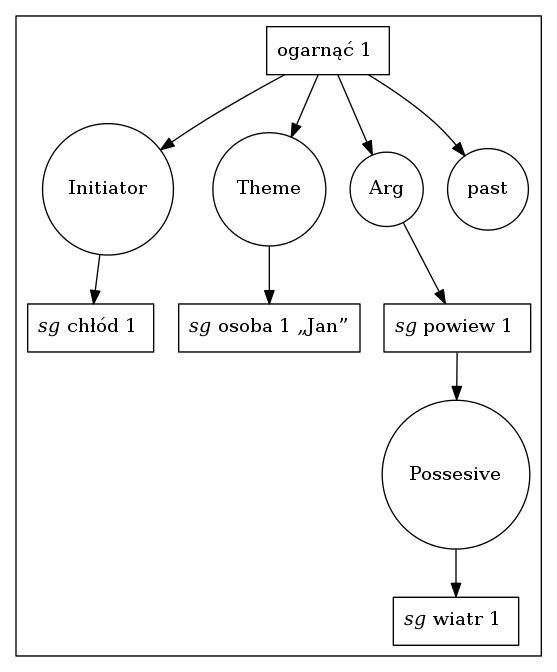
\includegraphics[scale=0.3]{metaopis_wiatr1.png}\\
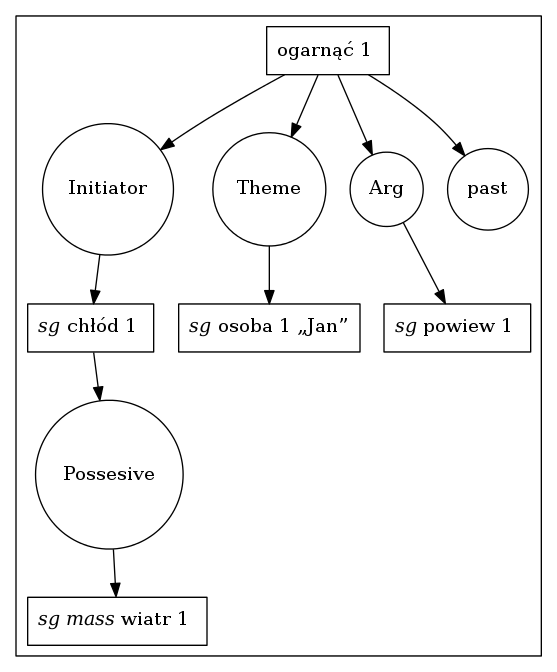
\includegraphics[scale=0.3]{metaopis_wiatr2.png}
\end{center}

\section{Inne przykłady}

% \begin{center}
% Modyfikowany przyimek {\it Ania schowała piłkę głęboko w szafie.}\\
% 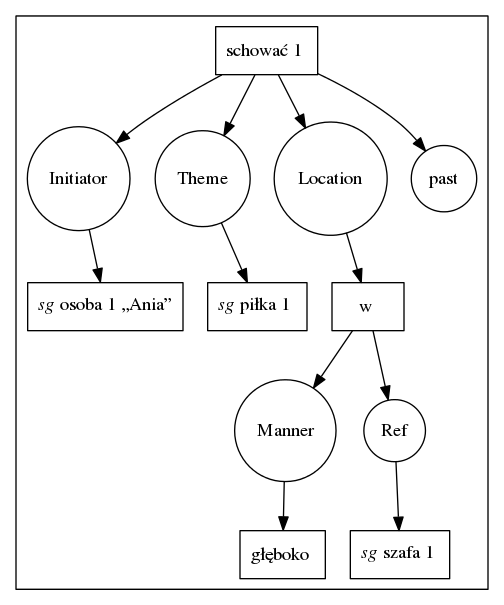
\includegraphics[scale=0.3]{metaopis_gleboko.png}\\
% Role tematyczne, przyimek niesemantyczny {\it Jaś wystosował petycję do urzędu.}\\
% 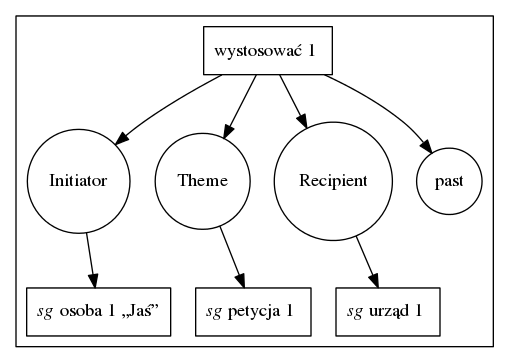
\includegraphics[scale=0.3]{metaopis_wystosowac.png}\\
% Rozpoznanie nazwy własnej dzięki preferencjom selekcyjnym,
% pojemniki i data. 
% {\it Kot odkupił 25 sierpnia 2015 samochód za 20000zł.}\\
% 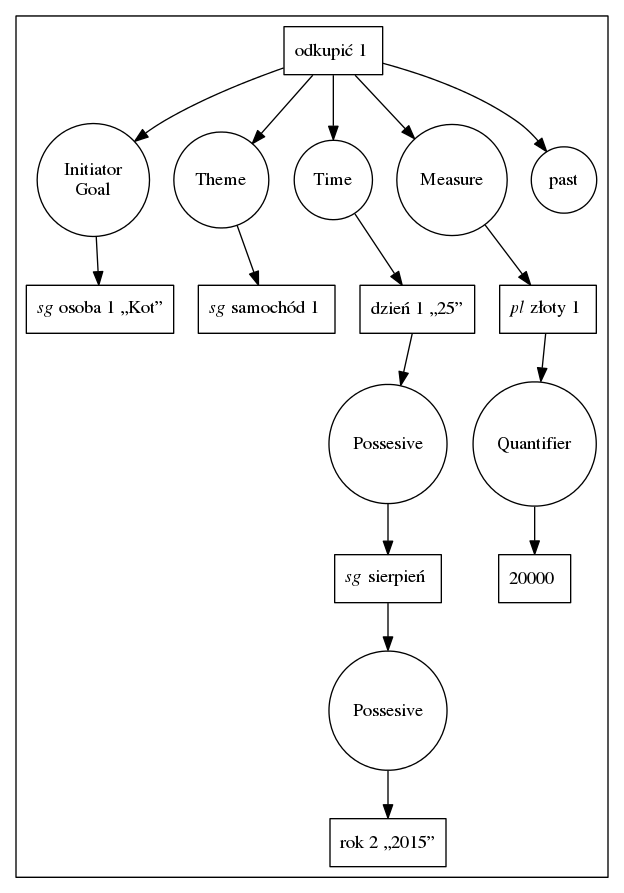
\includegraphics[scale=0.3]{metaopis_odkupic.png}\\
% Wykrycie rzadkiego leksemu, dzięki preferencjom selekcyjnym.
% {\it Chłopcy mają ulicę kwiatami.}\\
% 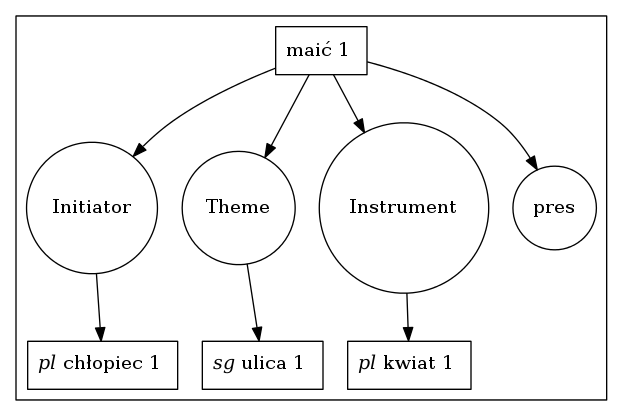
\includegraphics[scale=0.3]{metaopis_maic.png}\\
% Wielopoziomowe konteksty i mowa zależna
% {\it Jaś wierzy, że Marysia kłamała, kiedy powiedziała, że go nie kocha.}\\
% Rzeczowniki odnoszące się do pojęć:
% {\it Słonie są ssakami} vs {\it Słonie są gatunkiem}.\\
% Niejednoznaczność składniowa, kwantyfikator, indexical.
% {\it Codziennie jest tu opiekunka pani Gabrysia}\\
% \end{center}

\section{Zasoby istniejące i wymagające wytworzenia}
%TODO OPISAĆ

Źródła wiedzy: Walenty, informacje składniowe, zasoby semantyczne do utworzenia w Clarin 2
w szczególności kwantyfikatorowatość.

% TODO: niektóre przymiotniki i przysłówki (być może wszystkie)
% warto reprezentować jako leksemy rzeczownikowe, np. lwowsko i
% lwowski jako Lwów.

\end{document}




